\documentclass[8pt,xcolor=table,aspectratio=169]{beamer}

\usepackage{graphicx}
\usepackage{caption}
\usepackage{subcaption}
\usepackage{transparent}
\usepackage{epstopdf} %converting to PDF
\usepackage{multicol} 
\usepackage{animate}[2017/05/18]

\usepackage{makecell}

% \usepackage{pdfx}
 
% \usepackage[utf8]{inputenc}
% \usepackage[T1]{fontenc}
\usepackage[table]{xcolor}    % loads also »colortbl« 
%  \usepackage{enumitem}
% \usepackage{ucltemplate}
\usepackage{color}

\usepackage{comment}

\usepackage{tabularx} % make width of table columns evenly distributed (see http://tex.stackexchange.com/questions/60601/evenly-distributing-column-widths)
% \newcolumntype{Y}{>{\centering\arraybackslash}X}

% make entire row bold or italic in table
\newcommand\setrow[1]{\gdef\rowmac{#1}#1\ignorespaces}
\newcommand\clearrow{\global\let\rowmac\relax}
\clearrow


\usepackage{amssymb}% http://ctan.org/pkg/amssymb
\usepackage{pifont}% http://ctan.org/pkg/pifont
\newcommand{\cmark}{\ding{51}}%
\newcommand{\xmark}{\ding{55}}%


%\usepackage{pgfgantt} % for grantt charts
\usepackage{rotating}
\usepackage[graphicx]{realboxes}
\usepackage[export]{adjustbox}
\usepackage{array}

\usepackage{rotating}
% \usepackage{tabularx, booktabs} % make width of table columns evenly distributed (see http://tex.stackexchange.com/questions/60601/evenly-distributing-column-widths)
% \newcolumntype{Y}{>{\centering\arraybackslash}X}

\DeclareMathOperator*{\argmin}{arg\,min}
\DeclareMathOperator*{\argmax}{arg\,max}

\usepackage{tikz}
\usetikzlibrary{arrows,positioning, shapes.symbols,shapes.callouts,patterns,shapes,chains,calc,backgrounds,fadings}

% \definecolor{parCol}{rgb}{0.1, 0.1, 1}
% \definecolor{stCol}{rgb}{0.1, 0.6, 0.1}
% \definecolor{bothCol}{rgb}{0, 0.5, 0.5}

\definecolor{parCol}{rgb}{0, 0, 0}
\definecolor{stCol}{rgb}{0, 0, 0}
\definecolor{bothCol}{rgb}{0, 0, 0}
\definecolor{blue3}{HTML}{86B7FC} % med blue
\definecolor{blue1}{HTML}{B5F1FF} % light blue
\definecolor{blue2}{HTML}{E0F9FF} % very light blue

\newcolumntype{C}[1]{>{\centering\let\newline\\\arraybackslash\hspace{0pt}}m{#1}}

\setlength{\tabcolsep}{0.2em}

 
 %% OVERVIEW OF WORK SO FAR %%
 
%Information to be included in the title page:
\title{Machine learning for prediction and visualisation of brain diseases. Demonstration on Alzheimer's disease}
\author[Raz]{
R\u{a}zvan V. Marinescu\vspace{1em}}

\institute{\small{Medical Vision Group, Massachusetts Institute of Technology}

\vspace{0em}
\small{Centre for Medical Image Computing, University College London, UK}
}

\date{}

% logo of my university
\titlegraphic{
   \begin{figure}
   \begin{subfigure}{0.32\textwidth}
   \hspace{2em}
   
\includegraphics[height=1.0cm]{ucl_logo}
   \end{subfigure}
   \begin{subfigure}{0.32\textwidth}
   \centering
   
\includegraphics[height=1.0cm]{MIT_logo.png} 
   \end{subfigure}
   \begin{subfigure}{0.32\textwidth}
   \centering
   
\includegraphics[height=1.0cm]{pondLogo.png} 
   \end{subfigure}
   \end{figure}
   
   \tiny{Slides available online: https://people.csail.mit.edu/razvan}
}

\setbeamercolor{frametitle}{fg=black}
\setbeamercolor{author in head/foot}{fg=black, bg=white} 
\setbeamercolor{institute in head/foot}{fg=black, bg=white} 
\setbeamercolor{title in head/foot}{fg=black, bg=white}
\setbeamercolor{date in head/foot}{fg=black, bg=white}

\setbeamersize{text margin left=10pt,text margin right=10pt}
% \setbeamertemplate{frametitle}{
%     \vspace{0.9em}
%     \insertframetitle
% %     \vspace{-3em}
% }
\setbeamertemplate{frametitle}{%
    \vspace{0.5em}
    \usebeamerfont{frametitle}\insertframetitle%
    \vphantom{g}% To avoid fluctuations per frame
    %\hrule% Uncomment to see desired effect, without a full-width hrule
    \par% <-- added
    \hspace*{-\dimexpr0.5\paperwidth-0.5\textwidth}% <-- calculation of left margin width
    \rule[0.5\baselineskip]{\paperwidth}{0.4pt}%
}

\setbeamertemplate{footline}
{
  \vspace{-3em}
  \leavevmode%
   \rule{\paperwidth}{0.3pt}
  \hbox{%
  \begin{beamercolorbox}[wd=.3\paperwidth,ht=2.25ex,dp=1ex,center]{author in head/foot}%
    \usebeamerfont{author in head/foot}Razvan V. Marinescu
  \end{beamercolorbox}%
  \begin{beamercolorbox}[wd=.3\paperwidth,ht=2.25ex,dp=1ex,center]{institute in head/foot}%
    \usebeamerfont{institute in head/foot}razvan@csail.mit.edu
  \end{beamercolorbox}%
  \begin{beamercolorbox}[wd=.3\paperwidth,ht=2.25ex,dp=1ex,center]{institute in head/foot}%
    \usebeamerfont{institute in head/foot}https://people.csail.mit.edu/razvan/
  \end{beamercolorbox}%
%   \begin{beamercolorbox}[wd=.2\paperwidth,ht=2.25ex,dp=1ex,center]{title in head/foot}%
%     \usebeamerfont{title in head/foot}\insertsection
%   \end{beamercolorbox}%
  \begin{beamercolorbox}[wd=.10\paperwidth,ht=2.25ex,dp=1ex,right]{date in head/foot}%
    \usebeamerfont{date in head/foot}\insertshortdate{}\hspace*{2em}
    \insertframenumber{} / \inserttotalframenumber\hspace*{2ex}
  \end{beamercolorbox}}%
  \vskip0pt%
}

% \usepackage{beamerthemesplit}

\newcommand{\backupbegin}{
   \newcounter{finalframe}
   \setcounter{finalframe}{\value{framenumber}}
}
\newcommand{\backupend}{
   \setcounter{framenumber}{\value{finalframe}}
}


\makeatletter
\long\def\beamer@author[#1]#2{%
  \def\and{\tabularnewline}
  \def\insertauthor{\def\inst{\beamer@insttitle}\def\and{\tabularnewline}%
  \begin{tabular}{rl}#2\end{tabular}}%
  \def\beamer@shortauthor{#1}%
  \ifbeamer@autopdfinfo%
    \def\beamer@andstripped{}%
    \beamer@stripands#1 \and\relax
    {\let\inst=\@gobble\let\thanks=\@gobble\def\and{, }\hypersetup{pdfauthor={\beamer@andstripped}}}
  \fi%
}
\makeatother
\beamertemplatenavigationsymbolsempty
\setbeamertemplate{caption}[numbered]
\setbeamercolor{caption name}{fg=black}
\setbeamercolor{itemize item}{fg=black}
\setbeamercolor{itemize subitem}{fg=black}
\setbeamercolor{enumerate item}{fg=black}
\setbeamercolor{enumerate subitem}{fg=black}
\setbeamertemplate{enumerate item}[default]
\setbeamertemplate{enumerate subitem}[default]

\makeatletter
\let\@@magyar@captionfix\relax
\makeatother
\begin{document}
 
\section{Introduction}

\frame{\titlepage}
 
\setbeamerfont{frametitle}{size=\large}

\newcommand{\upgradeReportLoc}{../../upgrade_report}
\newcommand{\epsrcPresLoc}{\upgradeReportLoc/epsrcPres}
\newcommand{\jointModellingDiseaseLoc}{../../jointModellingDisease}
\newcommand{\pcaLongPaperLoc}{../../PCA_long_paper}
\newcommand{\voxFld}{../../voxelwiseDPM}
\newcommand{\tadpoleFld}{../../tadpole}
\newcommand{\diffEqModelFld}{../../diffEqModel}



\newcommand*{\pcaLongFigs}{\pcaLongPaperLoc/figures}


% \includeonlyframes{1-20}
%\includeonlyframes{current}



\newcommand{\ovHeight}{2cm}


% % TODO continue with overview, move into commands
\newcommand{\ovEBM}{
\begin{subfigure}{0.47\textwidth}
\centering
1. Modelled progression of PCA and tAD\\
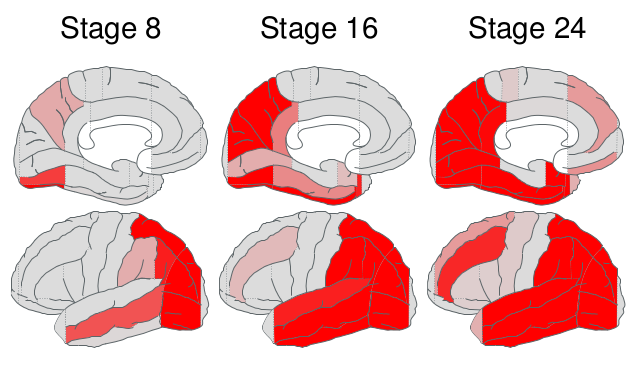
\includegraphics[height=\ovHeight]{ebm_thumb.png}
\end{subfigure}
}

\newcommand{\ovVWDPM}{
\begin{subfigure}{0.47\textwidth}
\centering
% \vspace{2.8em}
2. Developed Novel Spatio-temporal Model \\
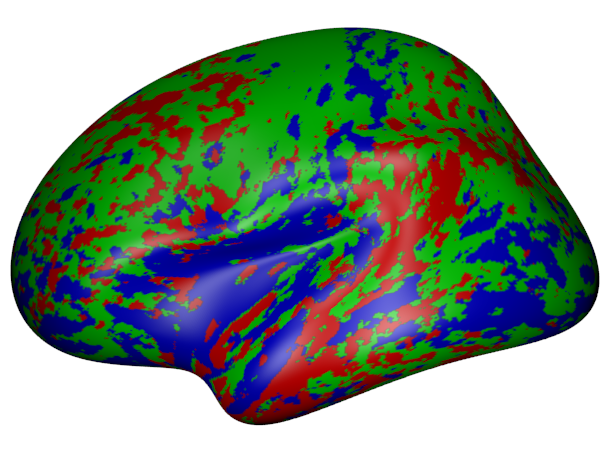
\includegraphics[height=\ovHeight]{\upgradeReportLoc/images/vwdpm/blend14_adniThavgFWHM0InithistCl3Pr0Ra1_VWDPMStd.png}
\end{subfigure}
}


\newcommand{\ovDKT}{
\begin{subfigure}{0.47\textwidth}
\centering
\vspace{1em}
3. Developed Transfer Learning Model\\ 
\vspace{0.5em}
\includegraphics[height=2.2cm]{\jointModellingDiseaseLoc/paper/figures/disease_knowledge_transfer.pdf}
\end{subfigure}
}


\newcommand{\ovTadpole}{
\begin{subfigure}{0.47\textwidth}
\centering
\vspace{-2em}
4. Meta-analysis of AD prediction algorithms\\
\vspace{1em}
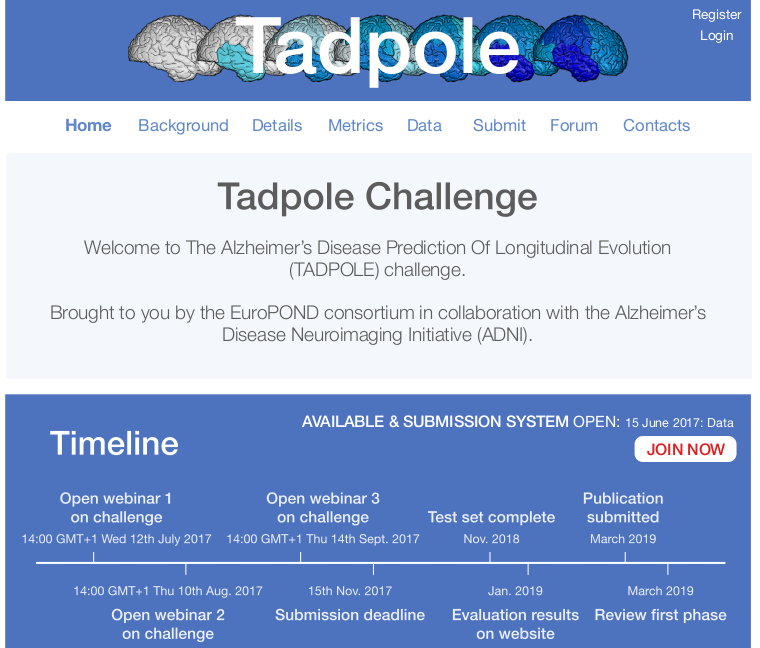
\includegraphics[height=1.2cm,valign=t]{\upgradeReportLoc/epsrcPres/tadpole} 
\end{subfigure}
}

\newcommand{\ovPainter}{
\begin{subfigure}{\textwidth}
\centering
\vspace{0.5em}
5. Created BrainPainter software\\
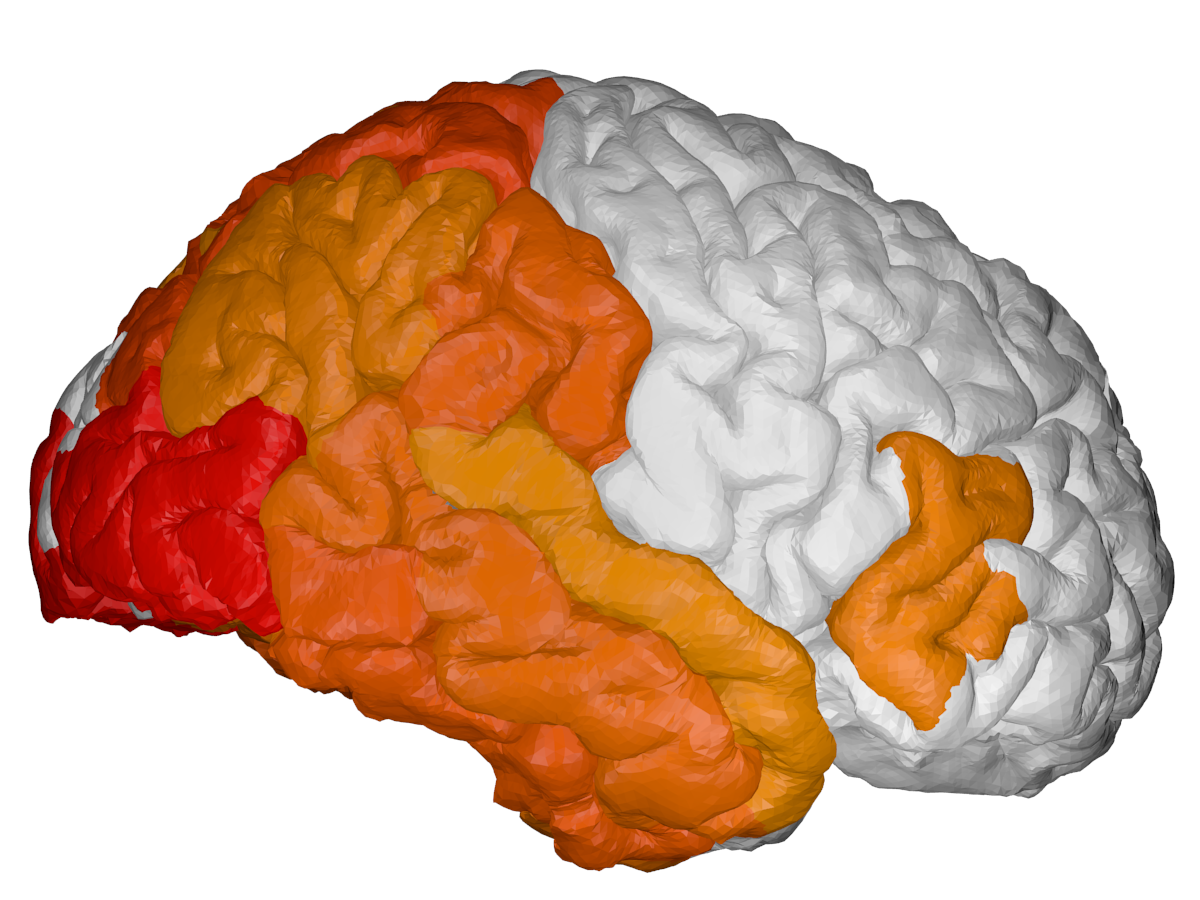
\includegraphics[height=1.5cm]{cortical-front_1}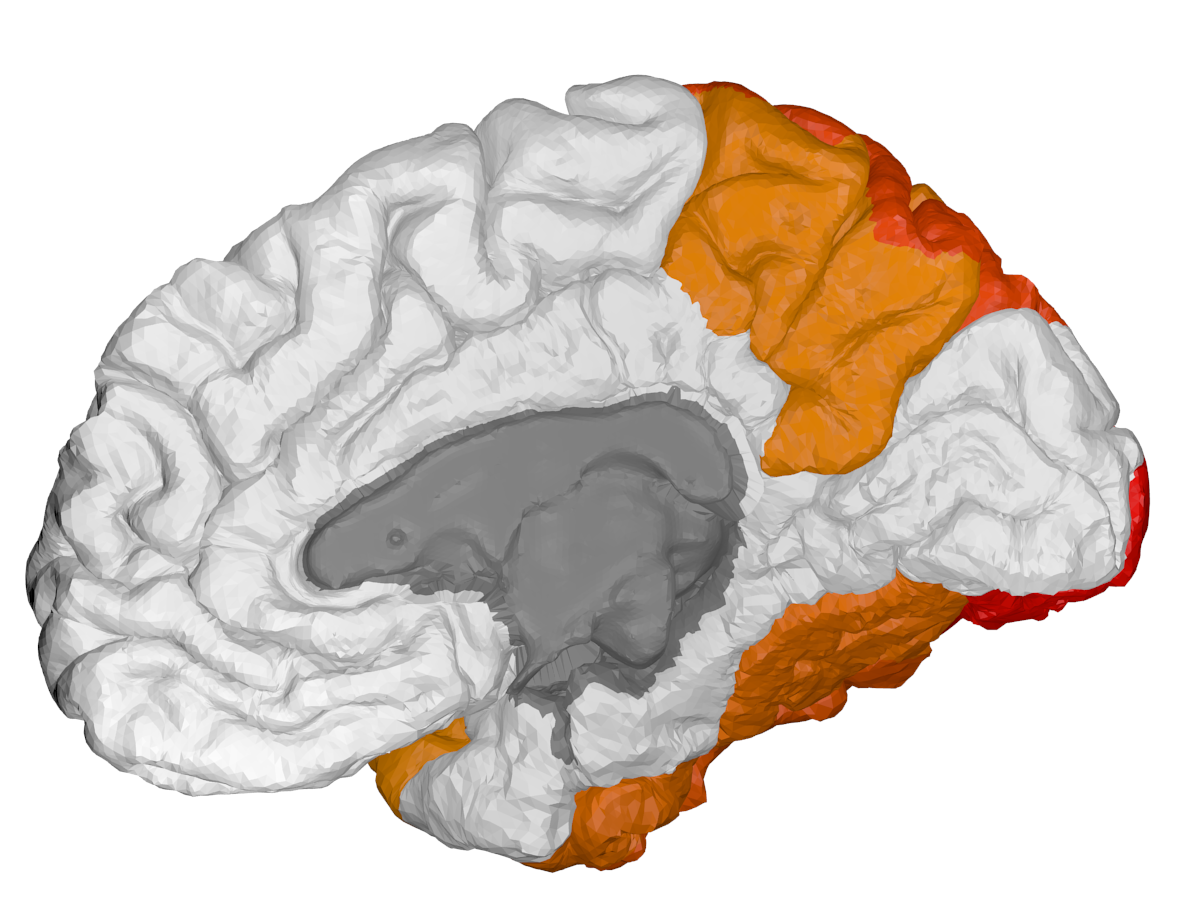
\includegraphics[height=1.5cm]{cortical-back_1}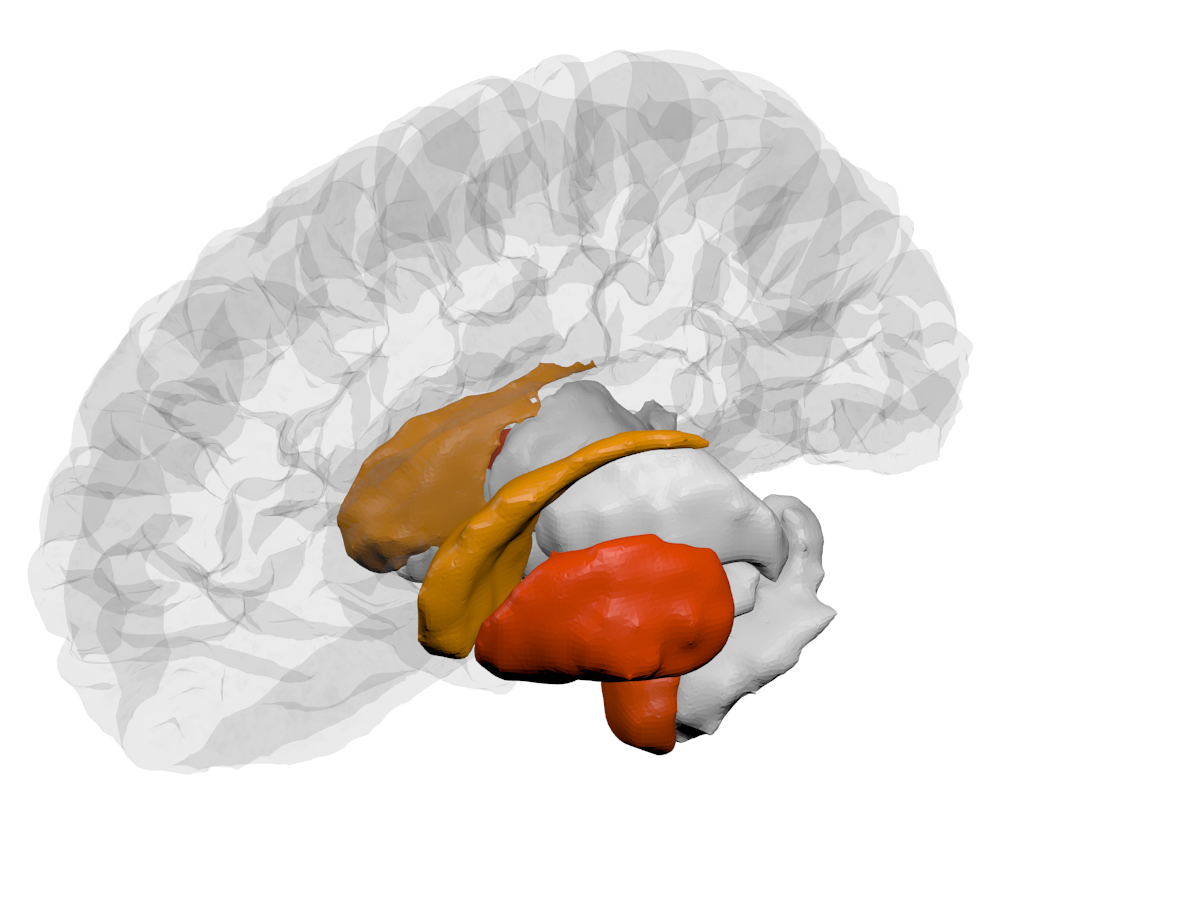
\includegraphics[height=1.5cm]{subcortical_1}
\end{subfigure}
}


\definecolor{light-gray}{gray}{0.6}



\begin{frame}{What to expect from my presentation}
 
 \begin{itemize}
 
  \onslide<1-> \item Why is prediction of Alzheimer's disease important? Why do drug trials fail?
  
  \vspace{2em}
  
  \onslide<2-> \item Which biomarkers can we predict, and which we cannot?
  
  \vspace{2em}
  
  \onslide<3-> \item What is the state-of-the-art in Alzheimer's prediction?
  
  \vspace{2em}
  
  \onslide<4-> \item What are the best algorithms? Should I use deep learning or not?
  
  \vspace{2em}
   
  \onslide<5-> \item Features: which ones are most informative? Do I need to pre-process those DTI scans, are MRIs not enough?
  
  \vspace{2em}
  
  \onslide<6-> \item How well do algorithms work on ``real data'', i.e. mimicking clinical trials?
  
  \vspace{2em}
  
  \onslide<7-> \item How can we visualise the progression of Alzheimer's disease? 
  
 \end{itemize}

\end{frame}



\begin{frame}
\frametitle{About me}

\begin{itemize}
  \item Grew up in Pitesti, Romania
  \item 2010-2014: Studied a 4-year MEng in Computer Science at Imperial College London
  \item 2014-2019: PhD in Medical Imaging at UCL (with Daniel Alexander)
  \item 2019-present: Postdoc in CSAIL at MIT (with Polina Golland)

  \begin{figure}
  \vspace{1em}
  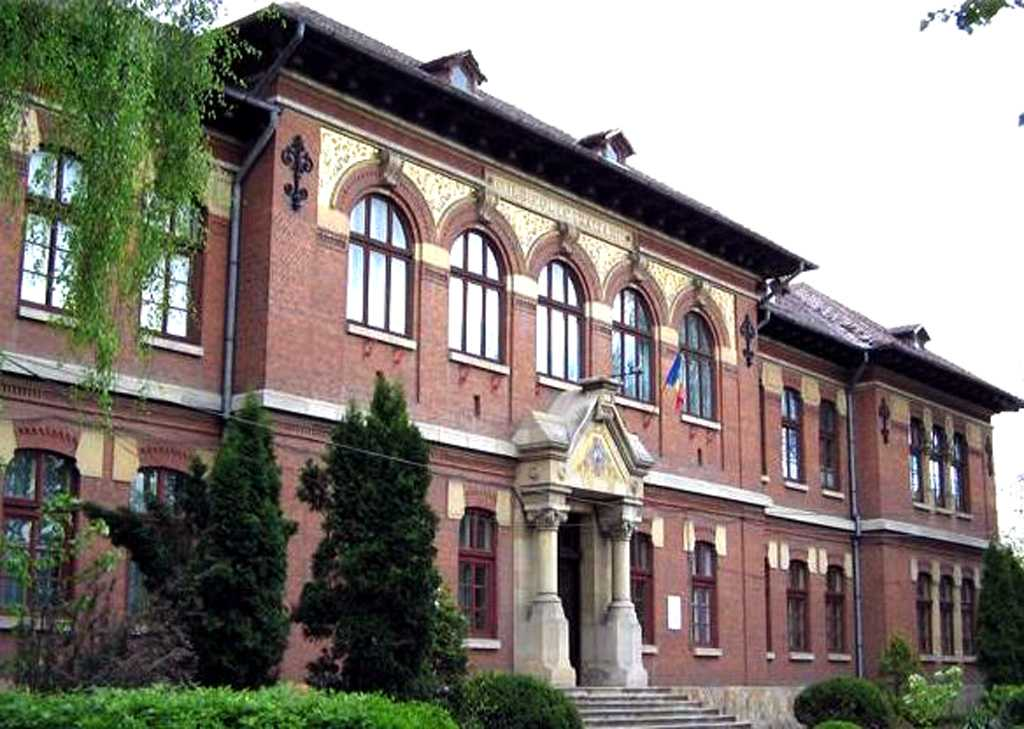
\includegraphics[height=2.7cm]{bratianu}\hspace{1em}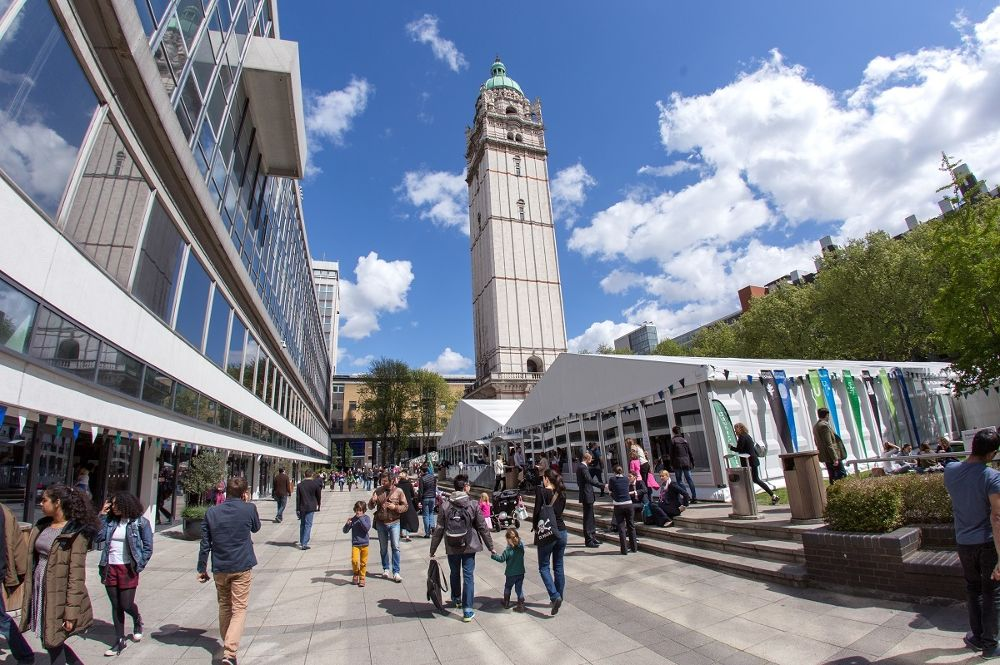
\includegraphics[height=2.7cm]{imperial.jpg}\hspace{1em}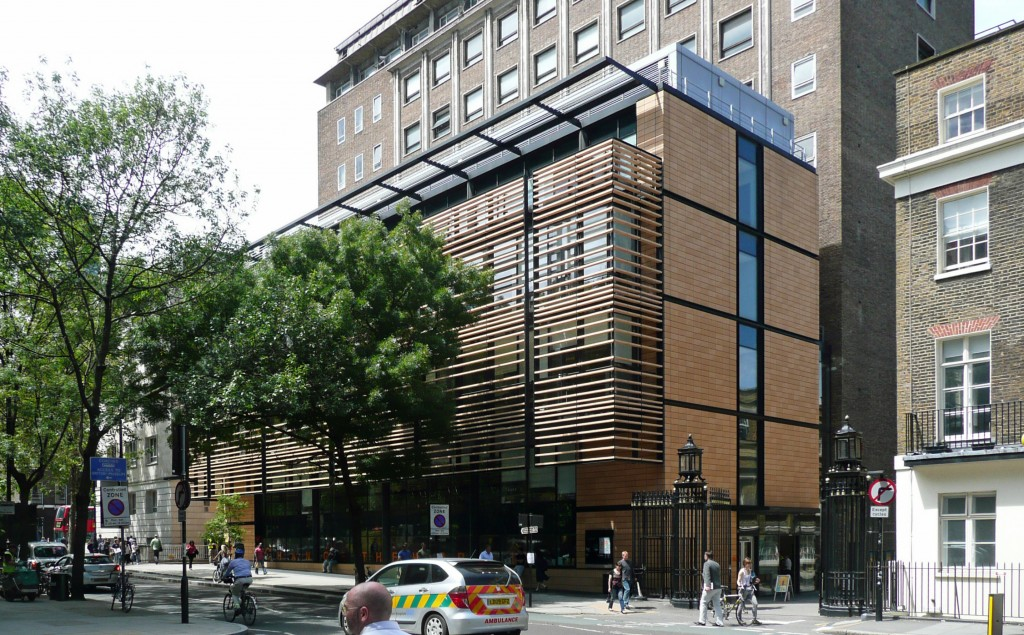
\includegraphics[height=2.7cm,trim=0 0 0 100,clip]{uclFrontEng.jpg}
  \end{figure}
 
 \vspace{1em}

 
 
%   \begin{figure}
%    \centering
% %     \hfill
%     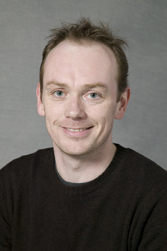
\includegraphics[height=2.2cm]{Danny-Alexander.jpeg}
%     \hspace{3em}
%     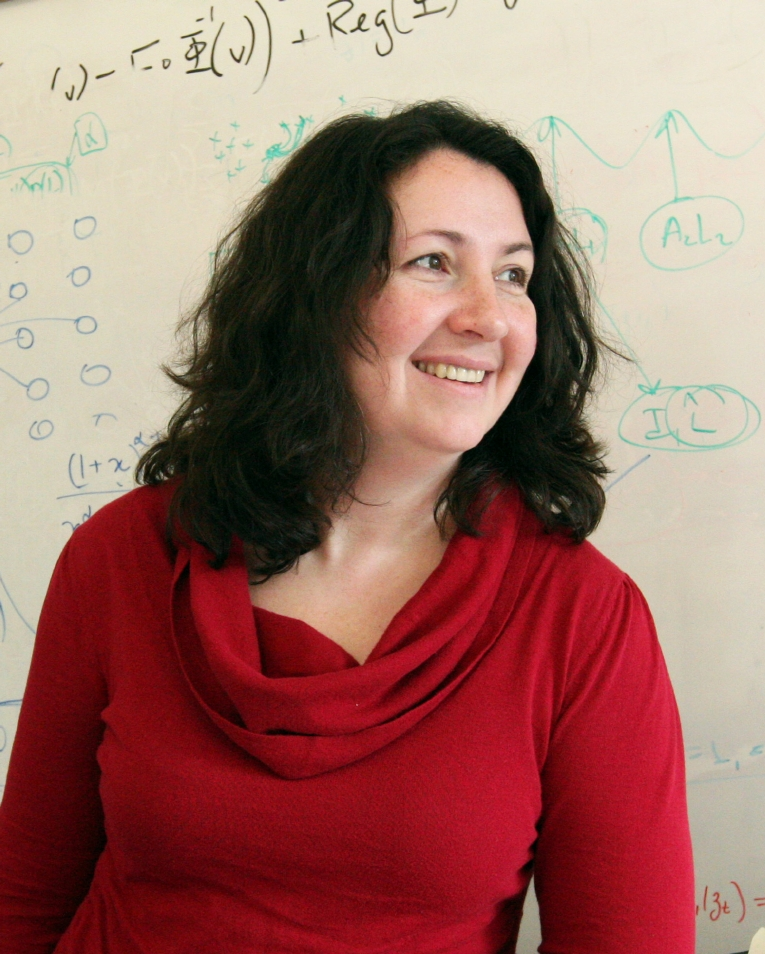
\includegraphics[height=2.2cm]{polina}  
% %     \hfill
%   \end{figure}



\end{itemize}

\end{frame}




\begin{frame}
\frametitle{Progression of Neurodegenerative Diseases (POND)}

\begin{figure}
\centering
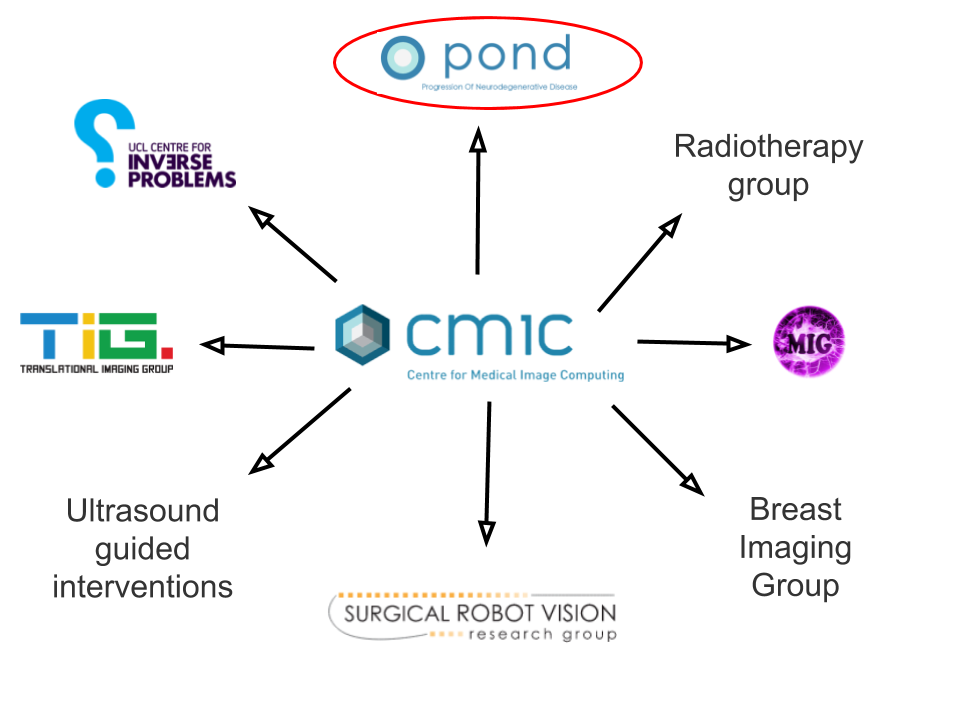
\includegraphics[height=8cm]{pond_diagram} 
\end{figure}



\end{frame}


\begin{frame}
\frametitle{POND Aim: Develop Computational Models for Disease Progression}

\newcommand{\mnpHeight}{3cm}

\vspace{-3em}
% \textbf{Background}:
% \onslide<1> \begin{itemize}
%   \item Aim: Develop computational models for disease progression
  
%   \vfill 
  
  \hspace{-2em}
  \begin{small}
  \begin{figure}[h]
  \centering
    \begin{minipage}[t][\mnpHeight][t]{0.49\linewidth}
  \centering
    \textbf{Event-Based Model}\\ \footnotesize{(Fontejin et al., Neuroimage, 2012)}\\    
    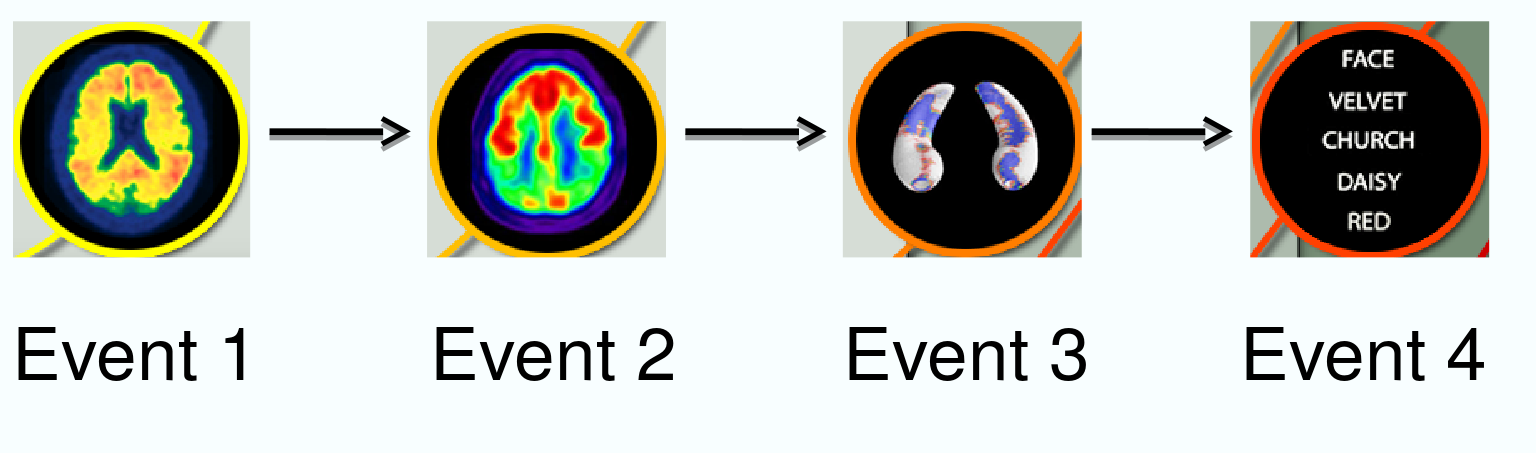
\includegraphics[width=0.9\textwidth,trim=0 0 0 0,clip]{ebm_openday}
      \vspace{1em}
%     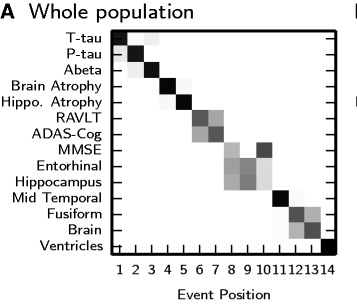
\includegraphics[width=0.4\textwidth]{young_positional_variance}
  \end{minipage}
  \begin{minipage}[t][\mnpHeight][t]{0.49\linewidth}
    \centering
    \textbf{Differential Equation Model}\\ \footnotesize{(Oxtoby et al., Brain, 2018)}
    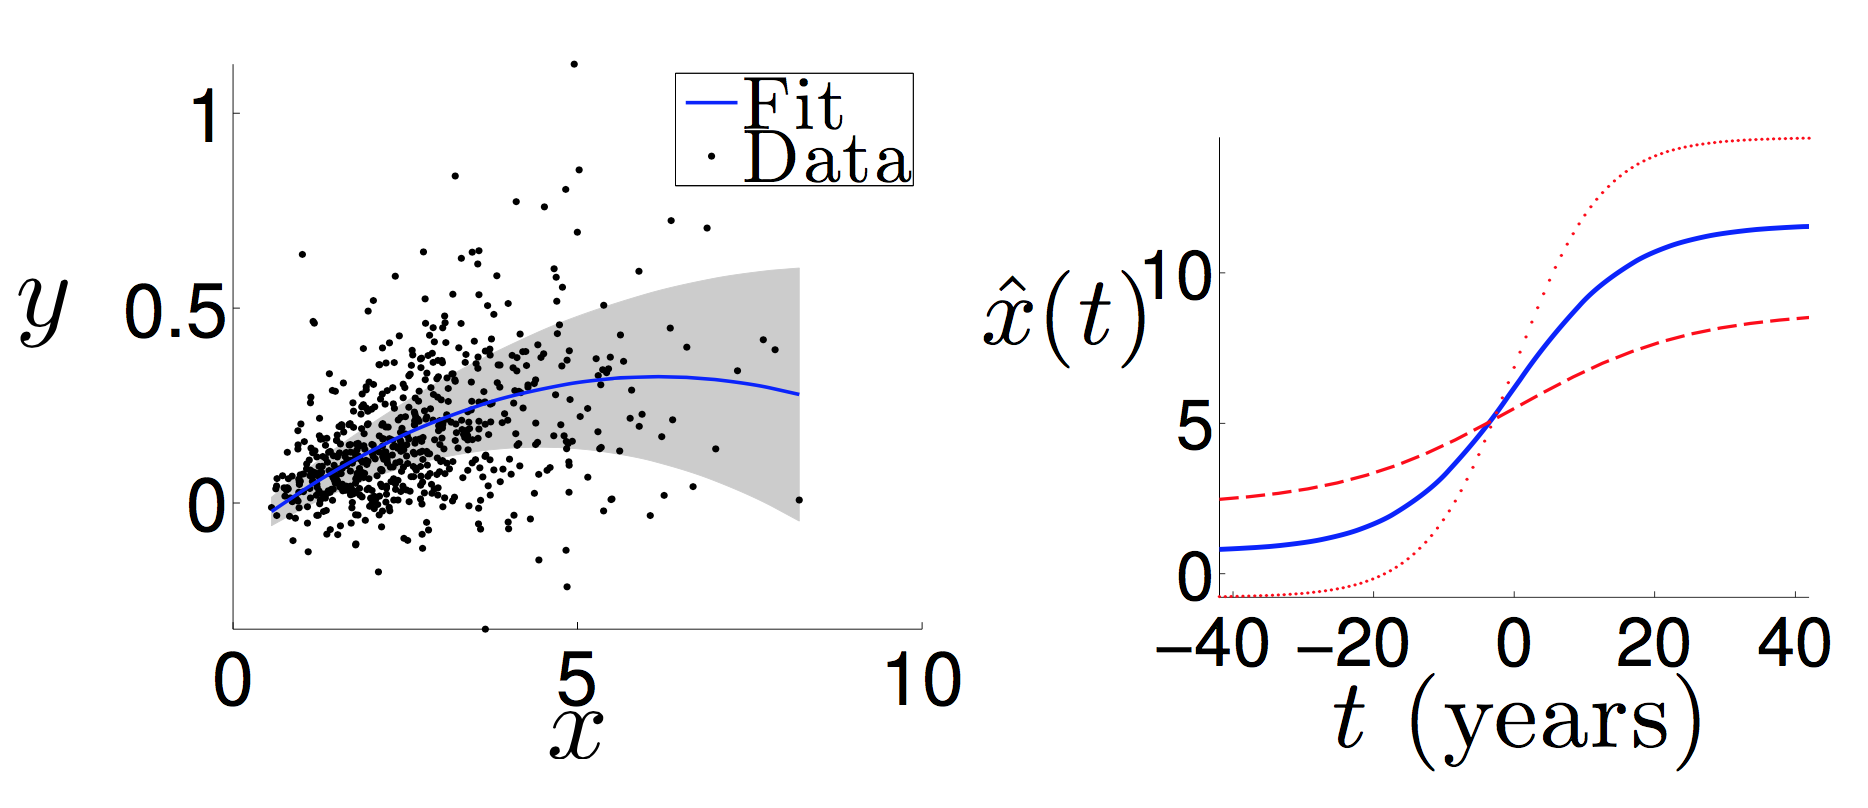
\includegraphics[width=0.9\textwidth,trim=0 0 0 0, clip]{dem_neil}
  \end{minipage}

  \vspace{2em}
  \begin{minipage}[t][\mnpHeight][t]{0.49\linewidth}
    \centering
    \textbf{Gaussian-Process Regression}\\ \footnotesize{(Lorenzi et al., IPMI, 2015)}
    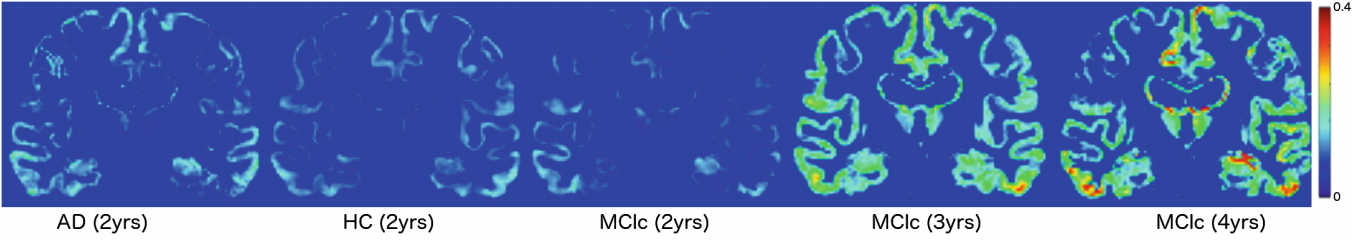
\includegraphics[width=0.9\textwidth,trim=0 0 0 0, clip]{lorenzi_ipmi2015}
    
    \vspace{2em}
    
  \end{minipage}
  \begin{minipage}[t][\mnpHeight][t]{0.49\linewidth}
    \centering
    \textbf{Subtype and Stage Inference}\\ \footnotesize{(Young et al., Nature Comms., 2018)}
    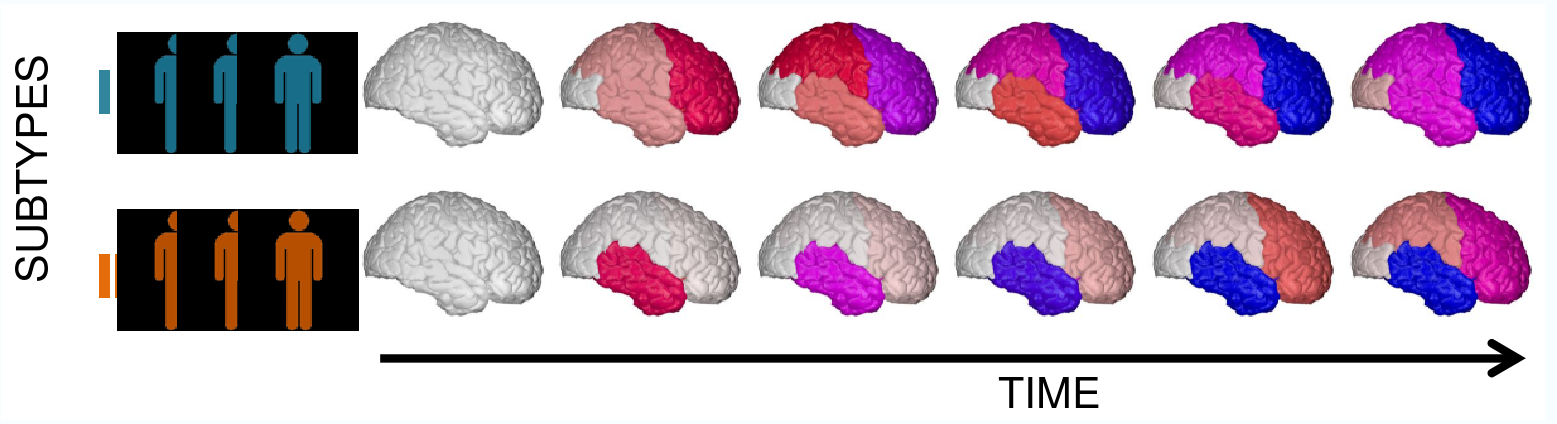
\includegraphics[width=0.9\textwidth]{sustain}
  \end{minipage}


  \end{figure}
  \end{small}
  
  \vspace{-2em}
  
% \end{itemize}


\end{frame}



\begin{frame}
\frametitle{POND Aim 2: Apply the Models to Distinct Neurodegenerative Diseases}

\newcommand{\mnpHeight}{3cm}

\vspace{-3em}
% \textbf{Background}:
% \begin{itemize}
%   \item 
  
%   \vfill 
  
  \hspace{-2em}
  \begin{small}
  \begin{figure}[h]
  \centering
  
      \begin{minipage}[t][\mnpHeight][t]{0.4\linewidth}
    \centering
    \textbf{typical Alzheimer's Disease}\\ \footnotesize{(Young et al., Nature Comms., 2018)}
    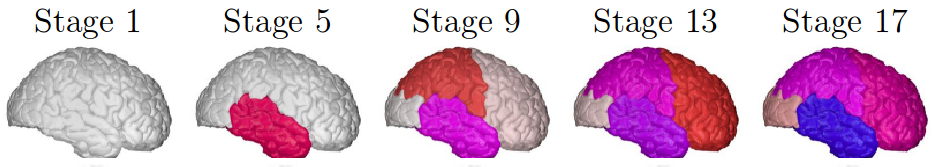
\includegraphics[width=0.9\textwidth]{young_progression.png}
  \end{minipage}
  \begin{minipage}[t][\mnpHeight][t]{0.4\linewidth}
    \centering
    \textbf{Familial Alzheimer's Disease}\\ \footnotesize{(Oxtoby et al., Brain, 2018)}
    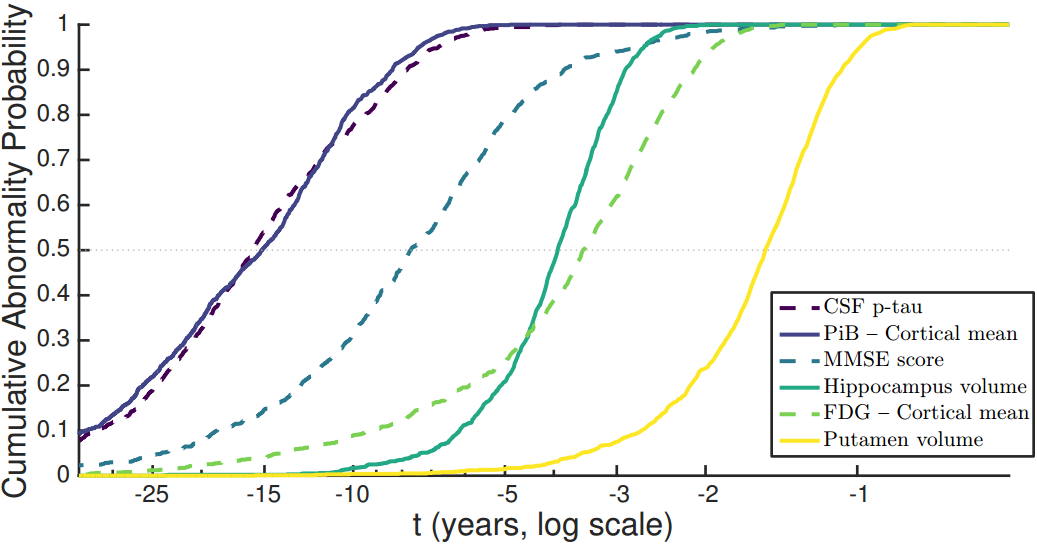
\includegraphics[width=0.7\textwidth,trim=0 0 0 0, clip]{neil_dian.png}
    
    \vspace{2em}
    
  \end{minipage}
  \vspace{2em}
  
    \begin{minipage}[t][\mnpHeight][t]{0.4\linewidth}
  \centering
    \textbf{Multiple sclerosis}\\ \footnotesize{(Eshaghi et al., Brain, 2017)}\\    
    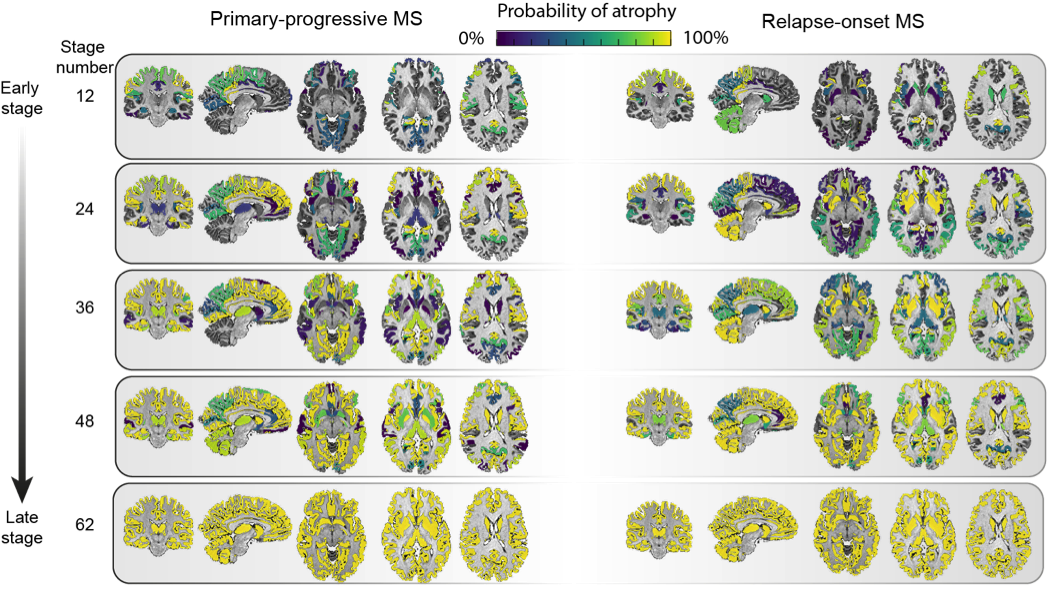
\includegraphics[width=0.9\textwidth,trim=0 0 0 0,clip]{ms_arman}
      \vspace{1em}
%     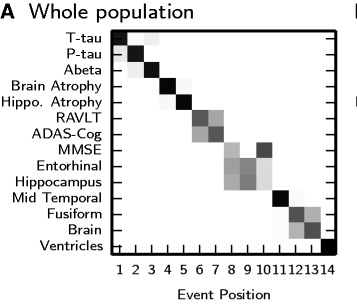
\includegraphics[width=0.4\textwidth]{young_positional_variance}
  \end{minipage}
  \begin{minipage}[t][\mnpHeight][t]{0.4\linewidth}
    \centering
    \textbf{Huntington's disease}\\ \footnotesize{(Wijeratne et al., Ann. Clin. Neurol;, 2018)}
    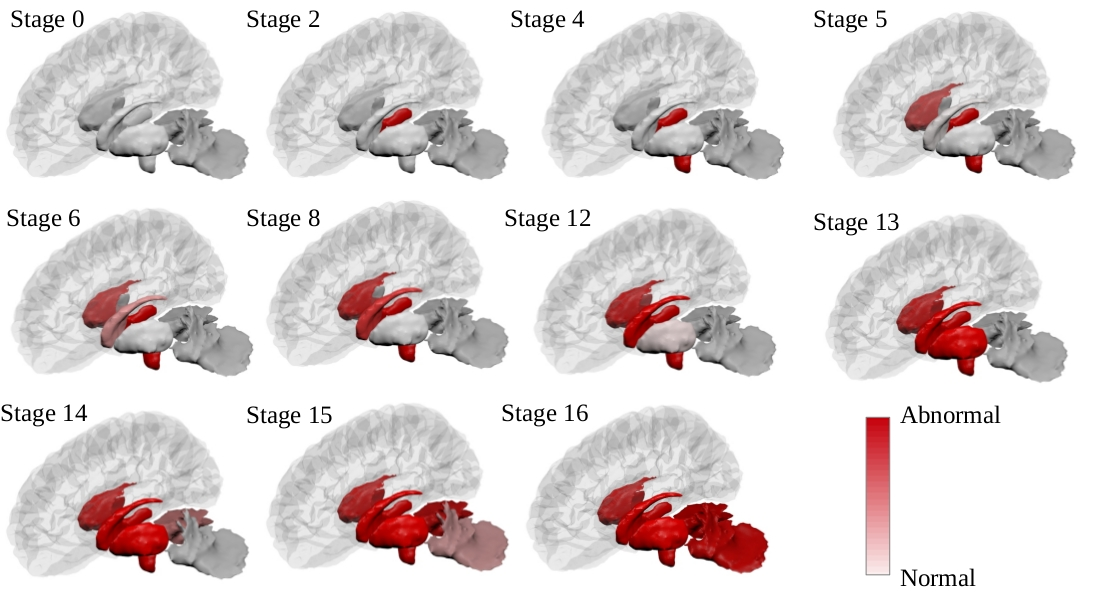
\includegraphics[width=0.9\textwidth,trim=0 0 0 0, clip]{hd_peter}
  \end{minipage}

\end{figure}
  \end{small}
  
%   \vspace{-2em}
  
% \end{itemize}



\end{frame}


\newcommand{\titleHigh}[1]{{\transparent{1.0}\textbf{#1}}} % title highlighting
\newcommand{\titleHighTwo}[1]{\underline{\textbf{#1}}} % title highlighting 2
\newcommand{\transpLevel}{0.4}

% \begin{frame}
% \frametitle{\textcolor{red}{Disease Progression} \textcolor{green}{Modelling} of \textcolor{blue}{Alzheimer's Disease} \textcolor{orange}{Subtypes}}
% 
% Title breakdown:\\
% \vspace{1em}
% \large{
% \textcolor{red}{Disease Progression} \textcolor{green}{Modelling} of \titleHighTwo{\textcolor{blue}{Alzheimer's Disease}} \textcolor{orange}{Subtypes}
% }
% 
% \vfill
% \vfill
% \vfill
% 
% \end{frame}



% \begin{frame}
% \frametitle{My PhD Aim}
% 
% \begin{enumerate}
%  \item Study the progression of pathology in Alzheimer's Disease (using existing models): 
%  
%   \begin{figure}
%   \centering
%   \vspace{1em}
%   \includegraphics[width=0.6\textwidth]{\epsrcPresLoc/brain_progression_16082017.png}
%   \end{figure}
%  
%  \vspace{1em}
% 
%  \item Develop novel disease progression models (DPMs)
%   \begin{equation}
%   \resizebox{0.6\columnwidth}{!}{% 
%   $p(X|S) = \prod_{j=1}^J \left[ \sum_{k=0}^N p(k) \left( \prod_{i=1}^k p\left(x_{s(i),j} | E_{s(i)} \right) \prod_{i=k+1}^N p\left(x_{s(i),j} | \neg E_{s(i)}\right) \right) \right]$
%   }
%   \end{equation}
% 
% %  \item Evaluate the performance of DPMs
% 
% \end{enumerate}
% 
% \end{frame}


\begin{frame}
\frametitle{Alzheimer's Disease is a Devastating Disease}

\vspace{-1em}
\begin{itemize}
 \item 46 million people affected worldwide
 
  \begin{figure}
 \centering
%   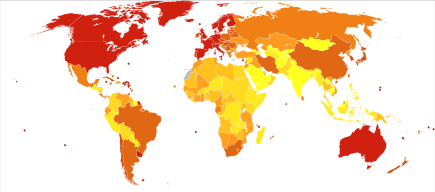
\includegraphics[height=3cm]{adPrelavence}
  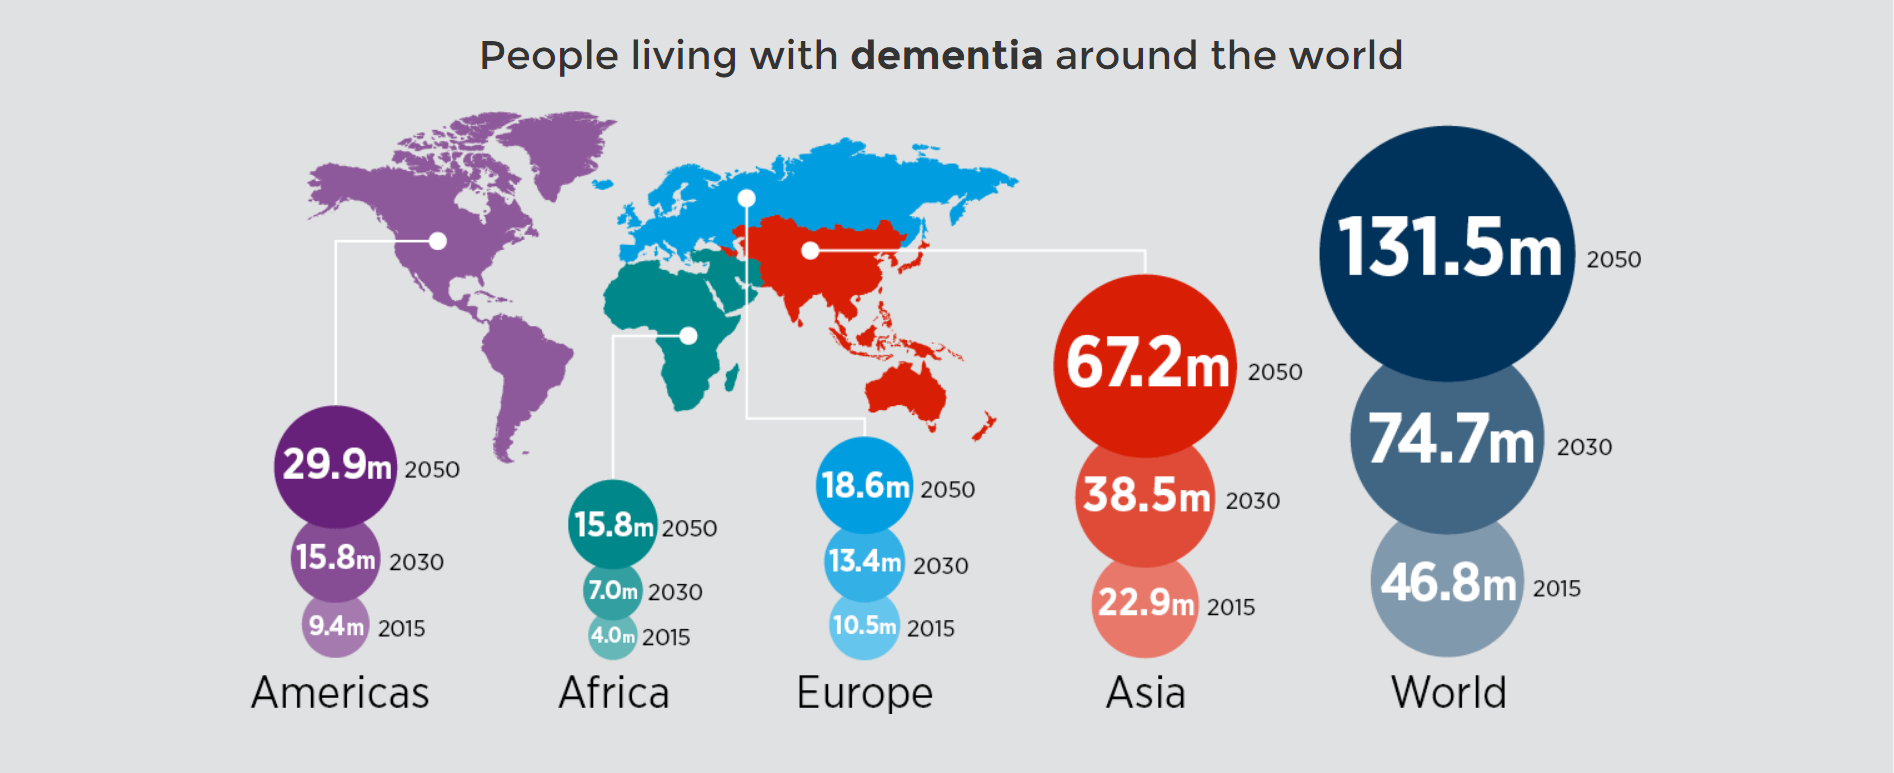
\includegraphics[height=4cm]{adPrevalanceIncreasing}
 \end{figure}
 
 \onslide<2-> \item No treatments available that stop or slow down cognitive decline
 \onslide<2-> \item Q: Why did clinical trials fail? A: Treatments were not administered early enough 
 \vspace{1em}
 \onslide<3-> \item Q: How can we then identify subjects \textbf{early} in order to administer treatments? 
 \onslide<3-> \item A: Build models that predict evolution of Alzheimer's biomarkers (i.e. biological markers) for at-risk subjects
  \vspace{1em}
 \onslide<4-> \item These models can help stage and refine cohorts in Alzheimer's clinical trials

\end{itemize}

\vspace{-1em}

\end{frame}

% Also say that we cannot build the model on age
\begin{frame}
\frametitle{Biomarker Evolution creates a Unique Disease Signature
that can be used for Staging Individuals in Clinical Trials}
% explain what are the challenges

\begin{figure}
\centering 
\vspace{-1em}
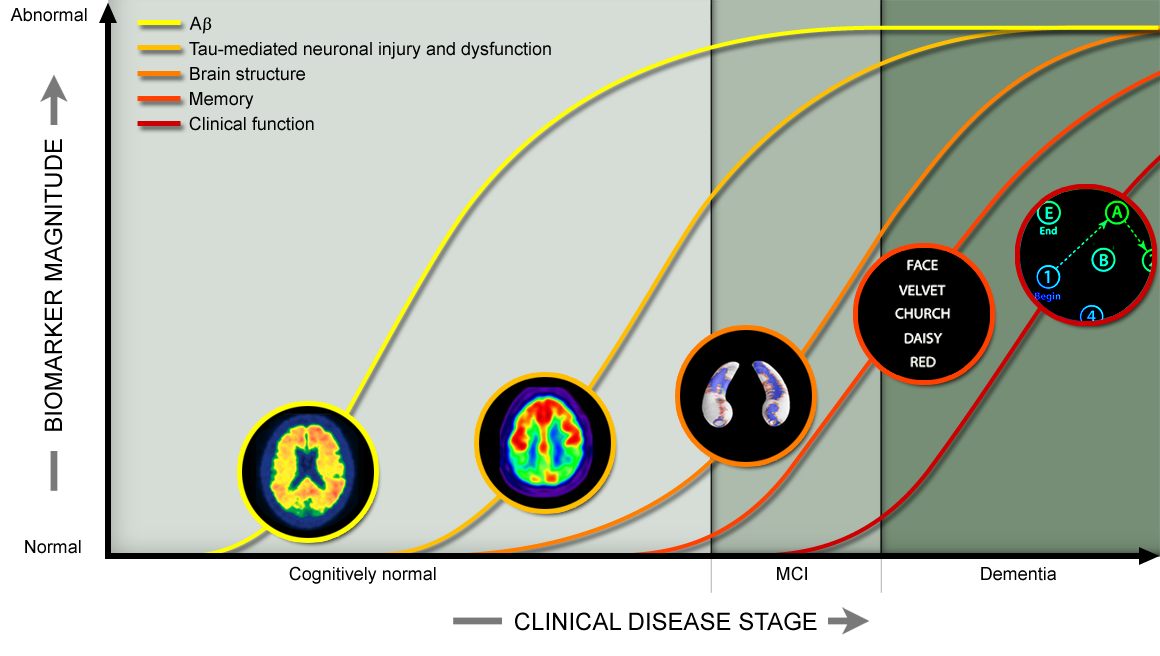
\includegraphics[height=5cm]{adniDiseaseProgression}
\hspace{-4em}Source: ADNI website 

\end{figure}


\begin{itemize}
 \item Accurate disease staging $\rightarrow$ better patient stratification
 \item Problem: This is a "hypothetical" (i.e. qualitative) disease progression model
 \item Why construct a quantitative model? 
\end{itemize}

\end{frame}


\section{Disease Progression Modelling}

% \begin{frame}
% \frametitle{\textcolor{red}{Disease Progression} \textcolor{green}{Modelling} of \textcolor{blue}{Alzheimer's Disease} \textcolor{orange}{Subtypes}}
% 
% Title breakdown:\\
% \vspace{1em}
% \large{
% \titleHighTwo{\textcolor{red}{Disease Progression} \textcolor{green}{Modelling}} of \textcolor{blue}{Alzheimer's Disease} \textcolor{orange}{Subtypes}
% }
% 
% \vfill
% \vfill
% \vfill
% 
% \end{frame}

\begin{frame}
\frametitle{Benefits of Quantitative Disease Progression Models}

\begin{overprint}
 \onslide<1>\begin{figure}
 \centering
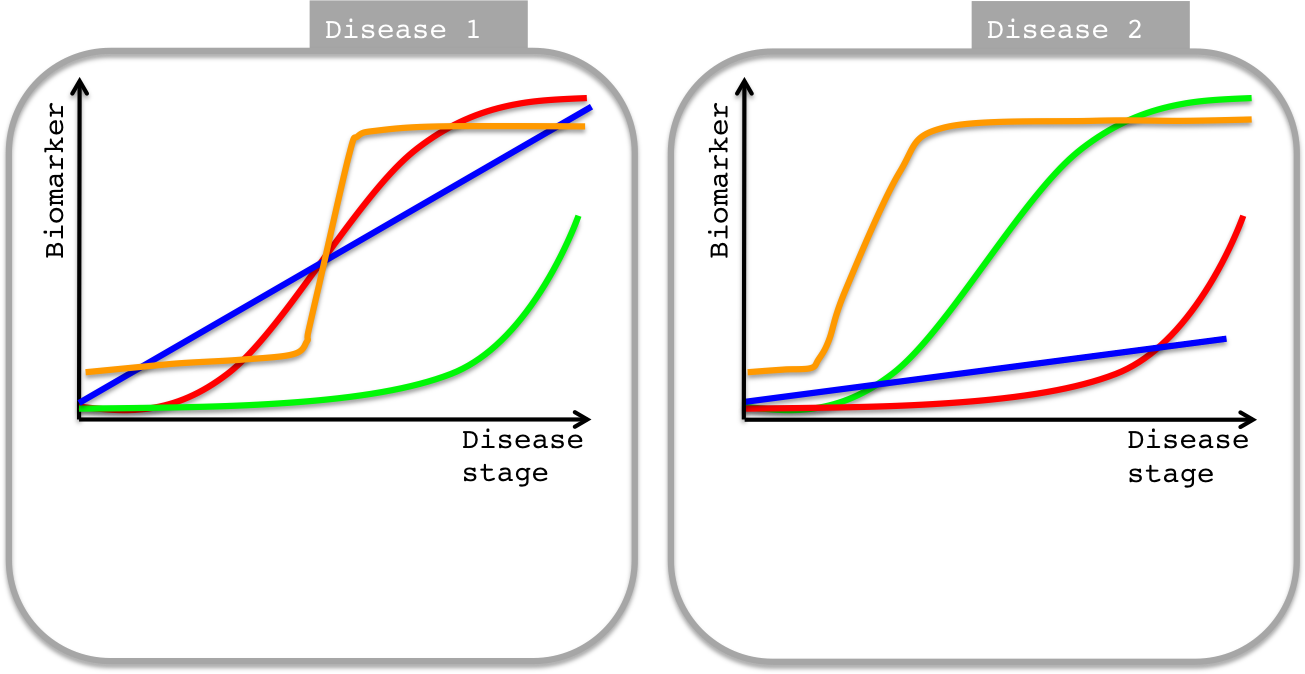
\includegraphics[height=5cm,trim=0 0 650 0,clip]{dpmDiffDiag1.png}
\end{figure}

\onslide<2> \begin{figure}
 \centering
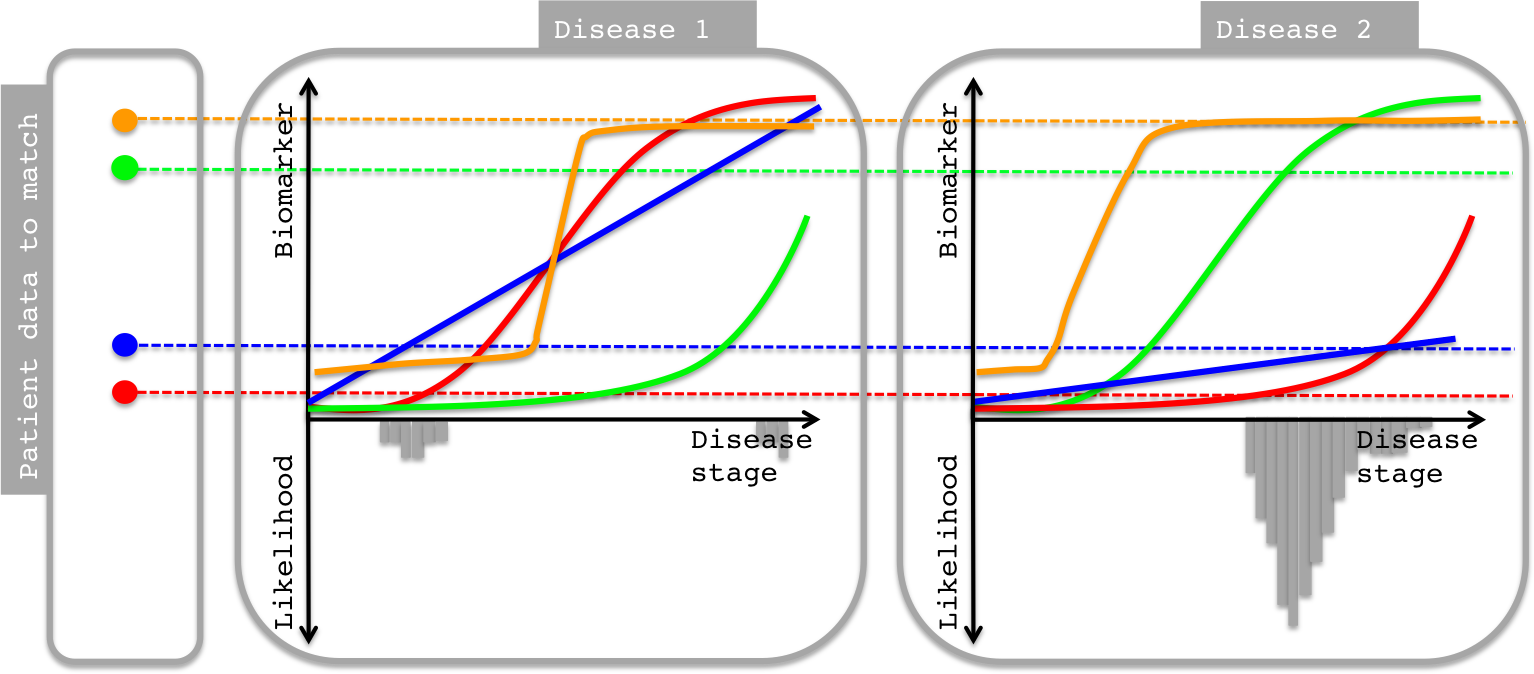
\includegraphics[height=5cm,trim=0 0 650 0,clip]{dpmDiffDiag2.png}
\end{figure}

\onslide<3-> \begin{figure}
 \centering
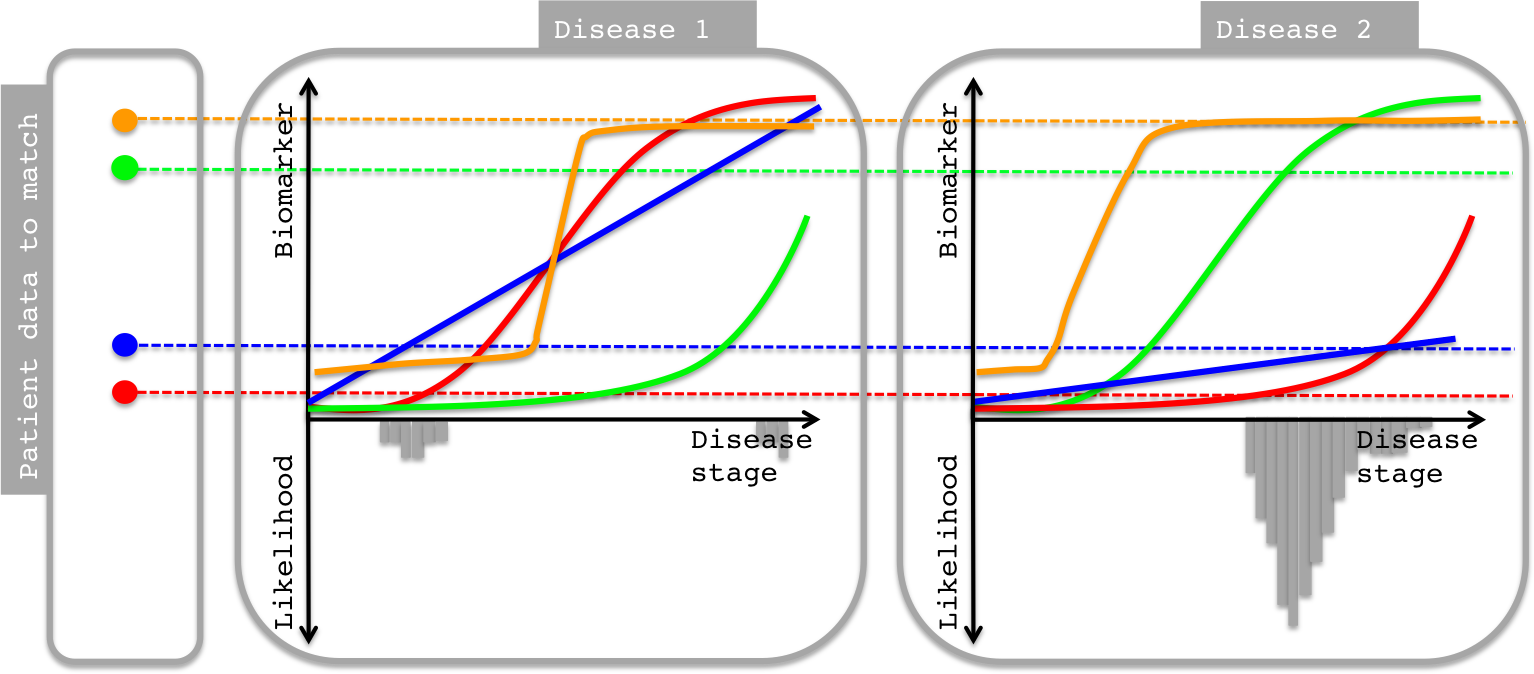
\includegraphics[height=5cm,trim=0 0 0 0,clip]{dpmDiffDiag2.png}
\end{figure}

\end{overprint}

\vspace{1em}
\begin{itemize}
 \onslide<1-> \item Basic biological insight
 \onslide<2-> \item Staging can help stratification in clinical trials
 \onslide<3-> \item Differential diagnosis and prognosis
 
%  \vspace{1em}
%  \onslide<4-> \item[] How can we build such a disease progression model?
\end{itemize}


 

\end{frame}


\begin{frame}[label=current]
\frametitle{My PhD Contributions}

\begin{figure}
\centering

\ovEBM
\ovVWDPM

\ovDKT
\ovTadpole

\ovPainter

\end{figure}

\end{frame}


\begin{frame}
\frametitle{Overview}

%% new slide

\begin{figure}
\centering

{\transparent{0.4}
\ovEBM
\ovVWDPM

\ovDKT}
\ovTadpole

\ovPainter

\end{figure}
\end{frame}



% \section{TADPOLE}


\definecolor{light-gray}{gray}{0.6}




\begin{frame}
\frametitle{TADPOLE is a Challenge to Predict the Progression of Individuals at Risk of AD}


\begin{columns}[t]
\begin{column}[t]{0.5\textwidth}

\begin{itemize}
 \item Identify people that will develop Alzheimer's disease (AD) over the next 1-5 years.

  \begin{itemize}
    \item Predict three target domains: clinical diagnosis, MRI (Ventricle Volume) and cognition (ADAS-Cog 13) 
  \end{itemize}

 \vspace{2em}

  \item Evaluation data on 219 subjects acquired by ADNI

 \vspace{2em}

 \item TADPOLE was entirely \textbf{prospective} -- evaluation data acquired after submission deadline: Nov 2017
 
 \vspace{2em}
 
 %\item TADPOLE stores forecasts and evaluates on follow-up data
 
 %\vfill
 
%  \item Why predict future evolution of AD?
%  \begin{itemize}
%   \item No treatments for AD currently available
%   \item Select the right subjects for AD clinical trials
%  \end{itemize}

\end{itemize}


\end{column}
\begin{column}[t]{0.5\textwidth}
%\vspace{-1em}
 \begin{figure}
\centering
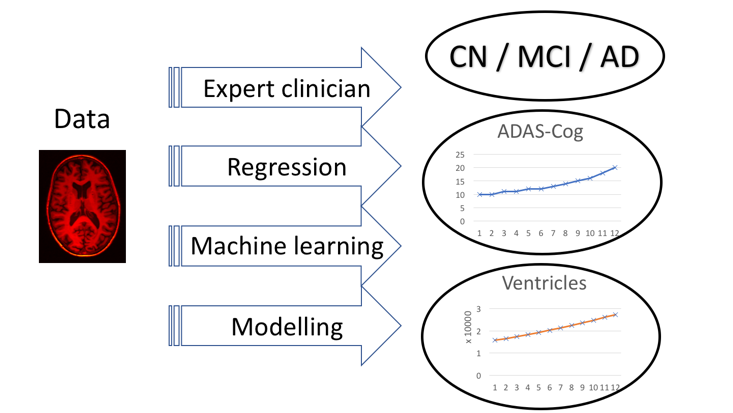
\includegraphics[height=4cm]{tadpole_diagram} 
\end{figure}
\vspace{-1em}

\end{column}

\end{columns}



\end{frame}



% \begin{frame}
% \frametitle{Alzheimer's Disease is a Devastating Disease}
% 
% \vspace{-1em}
% \begin{itemize}
% \item 46 million people affected worldwide
% 
%  \begin{figure}
% \centering
% %   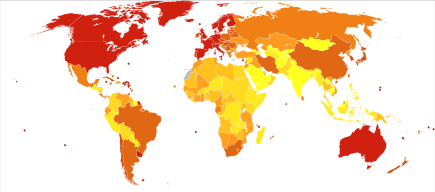
\includegraphics[height=3cm]{adPrelavence}
%  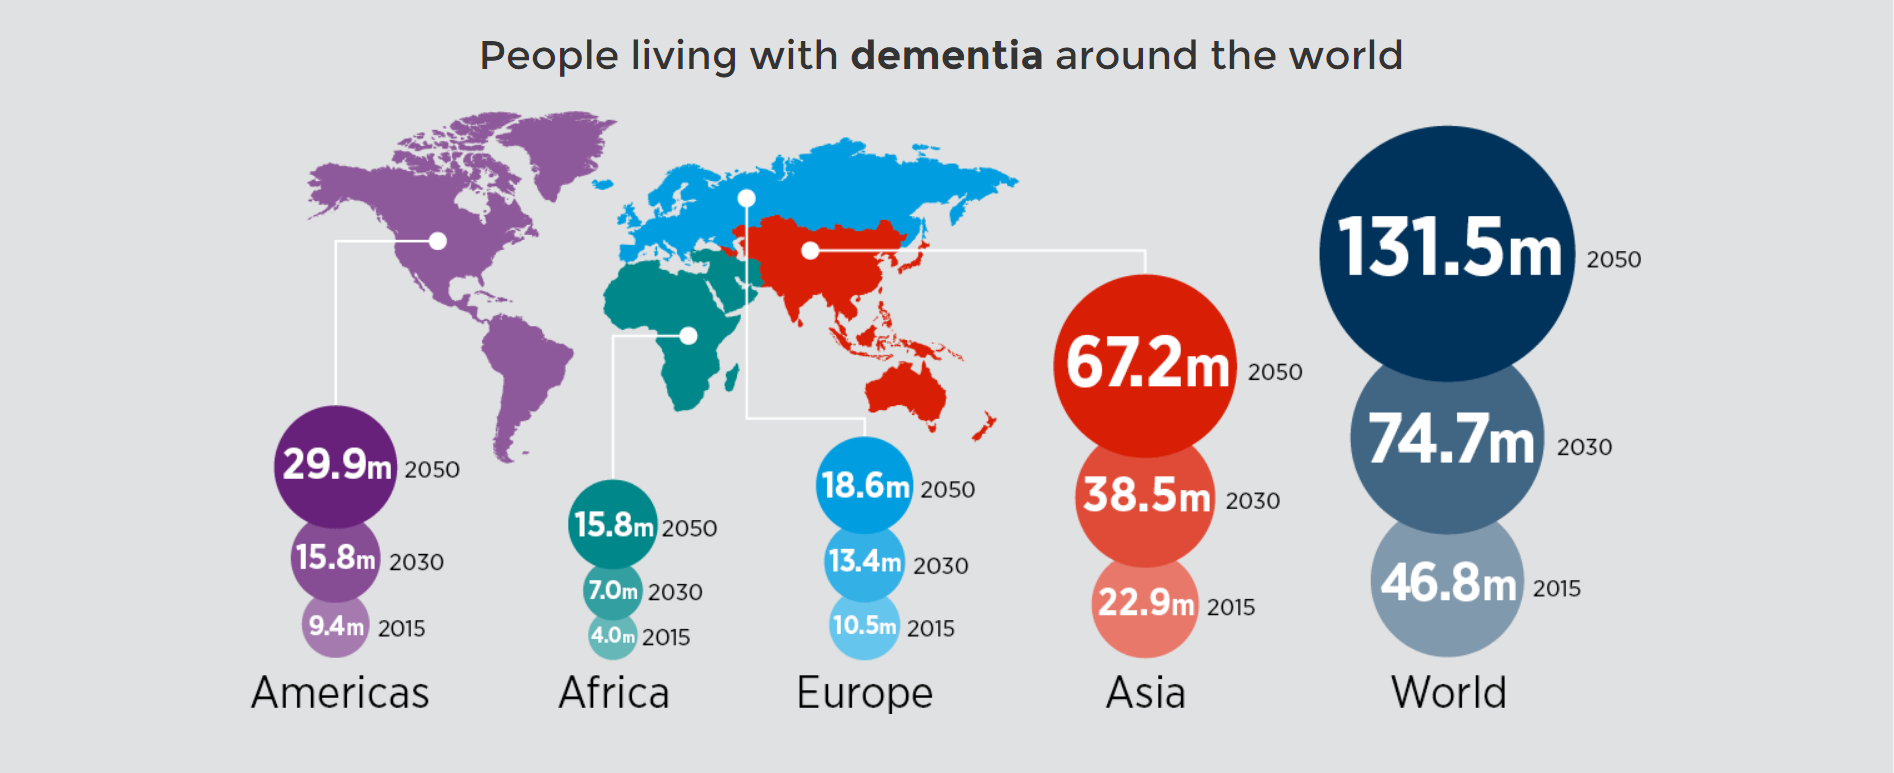
\includegraphics[height=4cm]{adPrevalanceIncreasing}
% \end{figure}
% 
% \onslide<2-> \item No treatments available that stop or slow down cognitive decline
% \onslide<2-> \item Q: Why did clinical trials fail? A: Treatments were not administered early enough 
% \vspace{1em}
% \onslide<3-> \item Q: How can we then identify subjects \textbf{early} in order to administer treatments? 
% \onslide<3-> \item A: Use prediction models that 
% 
% 
% \end{itemize}
% 
% \vspace{-1em}
% 
% \end{frame}



% \begin{frame}
%  \frametitle{Timeline}
%  
%  \begin{figure}
% \centering
% \begin{tikzpicture}
%     \draw (0, 0) node[inner sep=0] {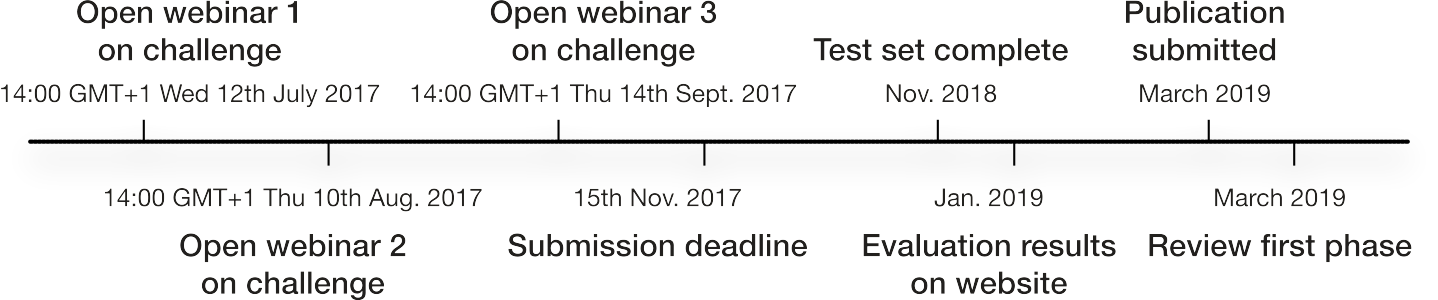
\includegraphics[width=0.9\textwidth]{Figure_Timeline_Black} };
%     \draw (2.4, -0.5) node {\small{\textcolor{red}{June 2019}}};
%     \draw (3.8, 0.3) node {\textcolor{red}{\small{November 2019}}};
%     \draw (4.4, -0.5) node {\textcolor{red}{\small{December 2019}}};
% \end{tikzpicture}
% \end{figure} 
%  
% \end{frame}




\setbeamerfont{frametitle}{size=\LARGE}

\definecolor{rosso}{RGB}{220,57,18}
\definecolor{giallo}{RGB}{255,153,0}
\definecolor{blu}{RGB}{102,140,217}
\definecolor{verde}{RGB}{16,150,24}
\definecolor{viola}{RGB}{153,0,153}


\makeatletter

\newcommand{\pythontexassign}[2]{%
  \expandafter\pythontexassign@i\expandafter{#2}{#1}}
\newcommand{\pythontexassign@i}[2]{%
  \pyc{#2=#1}}


\tikzstyle{chart}=[
    legend label/.style={font={\scriptsize},anchor=west,align=left},
    legend box/.style={rectangle, draw, minimum size=5pt},
    axis/.style={black,semithick,->},
    axis label/.style={anchor=east,font={\tiny}},
]

\tikzstyle{bar chart}=[
    chart,
    bar width/.code={
        \pgfmathparse{##1/2}
        \global\let\bar@w\pgfmathresult
    },
    bar/.style={very thick, draw=white},
    bar label/.style={font={\bf\small},anchor=north},
    bar value/.style={font={\footnotesize}},
    bar width=.75,
]

\tikzstyle{pie chart}=[
    chart,
    slice/.style={line cap=round, line join=round, very thick,draw=white},
    pie title/.style={font={\normalfont}},
    slice type/.style 2 args={
        ##1/.style={fill=##2},
        values of ##1/.style={}
    }
]

\pgfdeclarelayer{background}
\pgfdeclarelayer{foreground}
\pgfsetlayers{background,main,foreground}

\newcommand{\pie}[4][]{
    \begin{scope}[#1]
    \pgfmathsetmacro{\curA}{90}
    \pgfmathsetmacro{\r}{1}
    \def\c{(0,0)}
    \node[pie title] at (90:1.3) {#2};
    \pgfmathsetmacro{\sumAll}{0}
     \foreach \v/\s in{#3}{
        \pgfmathsetmacro{\sumAllTwo}{\v + \sumAll}
        \pgfmathsetmacro{\sumAll}{\sumAllTwo}
%         \expandafter\string\sumAll = \sumAll \par
%         \pgfmathprintnumber{\sumAll}
%         \pythontexassign{sumAll}{\sumAll}
    }
    \foreach \v/\s in{#3}{
	\pgfmathsetmacro{\argFour}{#4}
        \pgfmathsetmacro{\deltaA}{\v/\argFour * 360}
        \pgfmathsetmacro{\nextA}{\curA + \deltaA}
        \pgfmathsetmacro{\midA}{(\curA+\nextA)/2}

        \path[slice,\s] \c
            -- +(\curA:\r)
            arc (\curA:\nextA:\r)
            -- cycle;
        \pgfmathsetmacro{\d}{max((\deltaA * -(.5/50) + 1) , .5)}

        \begin{pgfonlayer}{foreground}
        \path \c -- node[pos=\d,pie values,values of \s]{$\v$} +(\midA:\r);
        \end{pgfonlayer}

        \global\let\curA\nextA
    }
    \end{scope}
}


\newcommand{\legend}[2][]{
    \begin{scope}[#1]
    \path
        \foreach \n/\s in {#2}
            {
                  ++(0,-10pt) node[\s,legend box] {} +(5pt,0) node[legend label] {\large{\n}}
            }
    ;
    \end{scope}
}


\begin{frame}
\frametitle{Submission statistics}


\vspace{-1em}
\begin{figure}
 33 teams from 12 countries\\
 \vspace{0.4em}
 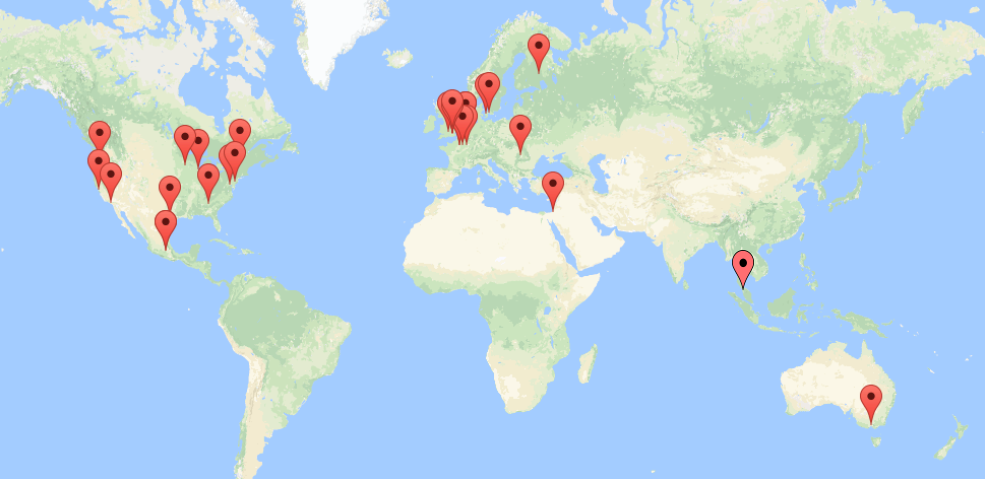
\includegraphics[height=4cm]{countriesMap2.png}
\end{figure}
\vspace{-1em}

\begin{figure}
 \centering
\begin{subfigure}{0.47\textwidth}
\centering
\begin{tikzpicture}
[
    pie chart,
    slice type={regression}{blu},
    slice type={machine}{rosso},
    slice type={dpm}{green},
    slice type={other}{yellow},
    pie values/.style={font={\Large}},
    scale=1.2
]
    \pie[xshift=0cm]{\Large{\begin{tabular}{c} Algorithms \end{tabular}} }{20/regression,23/machine,17/dpm,3/other}{63}
    \legend[shift={(1.4cm,1cm)}]{{Regression}/regression, {DPM}/dpm, {Other ML}/machine, {Other}/other}
\end{tikzpicture}
% \vspace{3.75em}
\end{subfigure}
\hspace{1em}
\begin{subfigure}{0.47\textwidth}
\centering
\begin{tikzpicture}
[
    pie chart,
    slice type={regular}{blu},
    slice type={school}{rosso},
    slice type={university}{green},
    slice type={benchmark}{orange},
    pie values/.style={font={\Large}},
    scale=1.2
]
    \pie[xshift=0cm]{\Large{\begin{tabular}{c} Teams \end{tabular}} }{50/regular,3/school, 11/university,4/benchmark}{68}
    \legend[shift={(1.4cm,1cm)}]{{Above PhD + Industry}/regular, {School}/school, {University}/university, {Benchmark}/benchmark}
\end{tikzpicture}
\end{subfigure}


\end{figure}

\end{frame}

\section{Methods}

%\begin{frame}
%\frametitle{Evaluation data}
%
%\begin{itemize}
% \item 219 test subjects with 223 cognitive visits and 150 MRI scans
% \item Test set was acquired after submission deadline
%\end{itemize}
%
%
%% \begin{table}
%% \centering
%%  \fontsize{7}{8}\selectfont
%% \begin{tabular}{|c|cccc|}
%% \hline
%% \textbf{Measure} &            \textbf{D1} &            \textbf{D2} &           \textbf{D3} &           \textbf{D4} \\
%% Subjects &          1667 &           896 &          896 &          219 \\
%% \hline
%% & \multicolumn{4}{c|}{\textbf{Cognitively Normal} }\\
%% Number (\% total) &   508 (30\%) &   369 (41\%) &  299 (33\%) &   94 (42\%) \\
%% Visits per subject &     8.3 $\pm$ 4.5 &     8.5 $\pm$ 4.9 &    1.0  $\pm$ 0.0 &    1.0  $\pm$ 0.2 \\
%% Age &    74.3  $\pm$ 5.8 &    73.6 $\pm$ 5.7 &   72.3 $\pm$ 6.2 &   78.4 $\pm$ 7.0 \\
%% Gender (\% male) &         48\% &         47\% &        43\% &        47\% \\
%% MMSE &    29.1  $\pm$ 1.1 &    29.0  $\pm$ 1.2 &   28.9  $\pm$ 1.4 &   29.1 $\pm$ 1.1 \\
%% Converters (\% total CN) &     18 (3.5\%) &      9 (2.4\%) &  - & - \\
%% \hline
%% & \multicolumn{4}{c|}{\textbf{Mild Cognitive Impairment} }\\
%% Number (\% total) &   841 (50.4\%) &   458 (51.1\%) &  269 (30.0\%) &   90 (41.1\%) \\
%% Visits per subject &     8.2 $\pm$ 3.7 &     9.1 $\pm$ 3.6 &    1.0 $\pm$ 0.0 &    1.1 $\pm$ 0.3 \\
%% Age &    73.0 $\pm$ 7.5 &    71.6 $\pm$ 7.2 &   71.9 $\pm$ 7.1 &   79.4 $\pm$ 7.0 \\
%% Gender (\% male) &         59.3\% &         56.3\% &        58.0\% &        64.4\% \\
%% MMSE &    27.6 $\pm$ 1.8 &    28.0 $\pm$ 1.7 &   27.6 $\pm$ 2.2 &   28.1 $\pm$ 2.1 \\
%% Converters (\% total MCI) &   117 (13.9\%) &     37 (8.1\%) &      -        &    9 (10.0\%) \\
%% \hline
%% & \multicolumn{4}{c|}{\textbf{Alzheimer's Disease}} \\
%% Number (\% total) &   318 (19.1\%) &     69 (7.7\%) &  136 (15.2\%) &   29 (13.2\%) \\
%% Visits per subject &     4.9 $\pm$ 1.6 &     5.2 $\pm$ 2.6 &    1.0 $\pm$ 0.0 &    1.1 $\pm$ 0.3 \\
%% Age &    74.8 $\pm$ 7.7 &    75.1 $\pm$ 8.4 &   72.8 $\pm$ 7.1 &   82.2 $\pm$ 7.6 \\
%% Gender (\% male) &         55.3\% &         68.1\% &        55.9\% &        51.7\% \\
%% MMSE &    23.3 $\pm$ 2.0 &    23.1 $\pm$ 2.0 &   20.5 $\pm$ 5.9 &   19.4 $\pm$ 7.2 \\
%% Converters (\% total AD) &       -        &      -         &        -      &    9 (31.0\%) \\
%%                 
%%  \hline
%% \end{tabular} 
%% %  \caption{Summary of TADPOLE datasets D1--D4. Each subject has been allocated to either Cognitively Normal, MCI or AD group based on diagnosis at the first available visit within each dataset.}
%% %  \label{tab:biomk_data_available}
%% \end{table}
%
%\begin{figure}
%\centering
% \includegraphics[height=4cm]{demographics_website}
%\end{figure}
%
%
%
%\end{frame}



\begin{frame}
\frametitle{Submission methods were very diverse}



\begin{table}
 \centering
 \fontsize{4}{6}\selectfont
 \begin{tabular}{c | >{\centering\arraybackslash}p{1.3cm} >{\centering\arraybackslash}p{1.2cm} >{\centering\arraybackslash}p{2cm} >{\centering\arraybackslash}p{2cm} >{\centering\arraybackslash}p{2cm}}
\textbf{Submission} & \textbf{Feature Selection}  & \textbf{Nr. of features} & \textbf{Missing data imputation} & \textbf{Diagnosis prediction} & \textbf{ADAS/Vent. prediction}\\
\Xhline{1.5\arrayrulewidth}
% Submission  & Feature selection & Number of features & Missing data imputation & Diagnosis prediction & ADAS/Vent. Prediction\\
AlgosForGood & manual & 16+5* & forward-filling & Aalen model & linear regression\\
Apocalypse & manual & 16 & population average & SVM & linear regression\\
ARAMIS-Pascal & manual & 20 & population average & Aalen model & -\\
ATRI-Biostat-JMM & automatic & 15 & random forest & random forest & linear mixed effects model\\
ATRI-Biostat-LTJMM & automatic & 15 & random forest & random forest & DPM\\
ATRI-Biostat-MA & automatic & 15 & random forest & random forest & DPM + linear mixed effects model\\
BGU-LSTM & automatic & 67 & none & feed-forward NN & LSTM\\
BGU-RF/ BGU-RFFIX & automatic & ~67+1340* & none & semi-temporal RF & semi-temporal RF\\
BIGS2 & automatic & all & Iterative Soft-Thresholded SVD & RF & linear regression\\
Billabong (all) & manual & 15-16 & linear regression & linear scale & non-parametric SM\\
BORREGOSTECMTY & automatic & ~100 + 400* & nearest-neighbour & regression ensemble & ensemble of regression + hazard models \\
BravoLab & automatic & 25 & hot deck & LSTM & LSTM\\
CBIL & manual & 21 & linear interpolation & LSTM & LSTM\\
Chen-MCW & manual & 9 & none & linear regression & DPM\\
CN2L-NeuralNetwork & automatic & all & forward-filling & RNN & RNN\\
CN2L-RandomForest & manual & $>$200 & forward-filling & RF & RF\\
CN2L-Average & automatic & all & forward-filling & RNN/RF & RNN/RF\\
CyberBrains & manual & 5 & population average & linear regression & linear regression\\
DIKU (all) & semi-automatic & 18 & none & Bayesian classifier/LDA + DPM & DPM\\
DIVE & manual & 13 & none & KDE+DPM & DPM\\
EMC1 & automatic & 250 & nearest neighbour & DPM + 2D spline + SVM & DPM + 2D spline\\
EMC-EB & automatic & 200-338 & nearest-neighbour & SVM classifier & SVM regressor\\
FortuneTellerFish-Control & manual & 19 & nearest neighbour & multiclass ECOC SVM & linear mixed effects model\\
% FortuneTellerFish-SuStaIn & manual & 19 & nearest neighbour & multiclass ECOC SVM + DPM & linear mixed effects model + DPM\\
% Frog & automatic & ~70+420* & none & gradient boosting & gradient boosting\\
% GlassFrog-LCMEM-HDR & semi-automatic & all & forward-fill & multi-state model & DPM + regression\\
% GlassFrog-SM & manual & 7 & linear model & multi-state model & parametric SM\\
% GlassFrog-Average & semi-automatic & all & forward-fill/linear & multi-state model & DPM + SM + regression\\
% IBM-OZ-Res & manual & Oct-15 & filled with zero & stochastic gradient boosting & stochastic gradient boosting\\
% ITESMCEM & manual & 48 & mean of previous values & RF & LASSO + Bayesian ridge regression\\
% lmaUCL (all) & manual & 5 & regression & multi-task learning & multi-task learning\\
% Mayo-BAI-ASU & manual & 15 & population average & linear mixed effects model & linear mixed effects model\\
% Orange & manual & 17 & none & clinician’s decision tree & clinician’s decision tree\\
% Rocket & manual & 6 & median of diagnostic group & linear mixed effects model & DPM\\
% SBIA & manual & 30-70 & dropped visits with missing data & SVM + density estimator & linear mixed effects model\\
% SPMC-Plymouth (all) & Automatic & 20 & none & ? & -\\
% SmallHeads-NeuralNetwork & automatic & 376 & nearest neighbour & deep fully -connected NN & deep fully -connected NN\\
% SmallHeads-LinMixedEffects & automatic & ? & nearest neighbour & - & linear mixed effects model\\
% Sunshine (all) & semi-automatic & 6 & population average & SVM & linear model\\
% Threedays & manual & 16 & none & RF & -\\
% Tohka-Ciszek-SMNSR & manual & ~32 & nearest neighbour & - & SMNSR\\
% Tohka-Ciszek-RandomForestLin & manual & ~32 & mean patient value & RF & linear model\\
% VikingAI (all) & manual & 10 & none & DPM + ordered logit model & DPM\\
... & ... & ... & ... & ... & ... \\
BenchmaskLastVisit & None & 3 & none & constant model & constant model\\
BenchmarkMixedEffect & None & 3 & none & Gaussian model & linear mixed effects model\\
BenchmarkMixedEffectAPOE & None & 4 & none & Gaussian model & linear mixed effects model\\
BenchmarkSVM & manual & 6 & mean of previous values & SVM & support vector regressor (SVR)
 \end{tabular}
%  \caption{Summary of benchmarks and top-3 methods used in the TADPOLE submissions. DPM -- disease progression model. ($^{\dagger}$) Aside from the three target biomarkers (*) Augmented features: e.g. min/max, trends, moments.}
%  \label{tab:submissions_desc}
\end{table}


\end{frame}



\begin{frame}
\frametitle{Prizes}

\begin{itemize}
 \item 30,000 GBP prize fund offered by sponsors:

\begin{figure}
\centering
 
\includegraphics[height=1.2cm]{alzsoc_logo}
 
\includegraphics[height=1.2cm]{alzassoc_logo}
 
\includegraphics[height=1.2cm]{alzresuk_logo}
\end{figure}

\vfill

 \item Prizes were split according into six categories:

\begin{table}
\centering
 \begin{tabular}{>{\centering\arraybackslash}m{1.5cm}  c  >{\centering\arraybackslash}m{2cm}}
\textbf{Prize amount} & \textbf{Outcome measure} & \textbf{Eligibility} \\
\hline
£5,000 & Diagnosis & all \\
£5,000 & Cognition & all\\
£5,000 & Ventricles & all\\
£5,000 & Overall best & all\\
£5,000 & Diagnosis & University teams\\
£5,000 & Diagnosis & High-school teams\\
\end{tabular}
\end{table}

\end{itemize}


\end{frame}

\definecolor{benchmarkCol}{rgb}{0.8,1,0.8}
\definecolor{univCol}{rgb}{0.8,0.8,1}
\definecolor{schoolCol}{rgb}{1,0.85,0.7}
\definecolor{randomCol}{gray}{0.85}
\definecolor{winnerCol}{rgb}{1,0.85,0.7}

\section{Results}

\begin{frame}{Results Outline}

\begin{itemize}
\item Prediction results:
\begin{itemize}
 \item Clinical diagnosis
  \item Ventricle volume
  \item Cognition
\end{itemize}

\vspace{2em}

\item Overall winners \& winning strategy

\vspace{2em}

% \item Consensus methods
% 
% \vspace{2em}

\item Results on limited dataset mimicking clinical trial

\vspace{2em}

\item Most informative features

\end{itemize}

\end{frame}

% \newcommand{\colbox}[2]{\colorbox{#1}{#2}}

\newcommand{\reducedstrut}{\vrule width 0pt height .9\ht\strutbox depth .9\dp\strutbox\relax}

\newcommand{\colbox}[2]{%
  \begingroup
  \setlength{\fboxsep}{0pt}%  
  \colorbox{#1}{\reducedstrut{#2}\/}%
  \endgroup
}

\begin{frame}
\frametitle{\textbf{Clinical Diagnosis prediction:} Winner algorithms achieve considerable gains over best benchmarks and state-of-the-art}

\begin{columns}[t]
\begin{column}[t]{0.6\textwidth}
 \begin{itemize}
  \item MAUC error reduced by 58\% compared to the \colbox{benchmarkCol}{best benchmark}
  
  \vspace{2em}
  
  \item \colbox{winnerCol}{Winner (Frog)} used a method based on gradient boosting (xgboost)
  
  \vspace{2em}
  
  \item TADPOLE algorithms pushed ahead the state-of-the-art:
  \begin{itemize}
    \item Best/29 algos in CADDementia challenge had a diagnosis MAUC of 0.78
    \item Best/15 algos (Morandi, NeuroImage, 2015) obtained AUC of 0.902
   \end{itemize}

  \vspace{2em}
  
  \item Full results on TADPOLE website: https://tadpole.grand-challenge.org/Results
   
\end{itemize}
\end{column}
\begin{column}[t]{0.4\textwidth}
 \begin{figure}
\centering
\begin{table}
\fontsize{6}{8}\selectfont
\begin{tabular}{l|c|c}
\Xhline{2.5\arrayrulewidth}
                    \textbf{Team Name} & \textbf{RANK MAUC} &   \textbf{MAUC} \\
\Xhline{2.5\arrayrulewidth}
  \rowcolor{winnerCol}   Frog &         1 &  0.931 \\
                    Threedays &         2 &  0.921 \\
                    EMC-EB &         3 &  0.907  \\
                GlassFrog-SM &       4-6 &  0.902 \\
            GlassFrog-Average &       4-6 &  0.902 \\
        GlassFrog-LCMEM-HDR &       4-6 &  0.902 \\
                    Apocalypse &         7 &  0.902 \\
                    EMC1-Std &         8 &  0.898  \\
                        CBIL &         9 &  0.897  \\
            CN2L-RandomForest &        10 &  0.896  \\
%                 EMC1-Custom &        11 &  0.892 \\
%                         BGU-LSTM &        12 &  0.883 &  0.779 \\
%     DIKU-GeneralisedLog-Custom &        13 &  0.878 &  0.790 \\
%         DIKU-GeneralisedLog-Std &        14 &  0.877 &  0.790 \\
%                     ARAMIS-Pascal &        15 &  0.876 &  0.850 \\
%              VikingAI-Sigmoid &        16 &  0.875 &  0.760 \\
%  Tohka-Ciszek-RandomForestLin &        17 &  0.875 &  0.796 \\
%                    IBM-OZ-Res &        18 &  0.868 &  0.766 \\
%                 BORREGOTECMTY &        19 &  0.866 &  0.808 \\
%             VikingAI-Logistic &        20 &  0.865 &  0.754 \\



%                    lmaUCL-Std &        21 &  0.859 &  0.781 \\
%             lmaUCL-Covariates &        22 &  0.852 &  0.760 \\
%                                     &       ... &         \\
%                 Chen-MCW-Stratify &        23 &  0.848 \\
                           ...          &       ... &   ...      \\
%                  AlgosForGood &        24 &  0.847 &  0.810 \\
%         Sunshine-Conservative &        25 &  0.845 &  0.816 \\
%                 lmaUCL-halfD1 &        26 &  0.845 &  0.753 \\
%                  CN2L-Average &        27 &  0.843 &  0.792 \\
%                        BGU-RF &        28 &  0.838 &  0.673 \\

%   \rowcolor{schoolCol} Chen-MCW-Std &        29 &  0.836 &  0.778 \\

\rowcolor{benchmarkCol} BenchmarkSVM &        30 &  0.836  \\
%     FortuneTellerFish-Control &        31 &  0.834 &  0.692 \\
%                     BGU-RFFIX &        32 &  0.831 &  0.673 \\
%                  Sunshine-Std &        33 &  0.825 &  0.771 \\
                      ...           &       ... &  ...     \\
%                     CyberBrains &        34 &  0.823 \\
% \rowcolor{benchmarkCol} BenchmarkMixedEffectsAPOE &        35 &  0.822 &  0.749 \\
%                                 &       ... &        \\   
%       DIKU-ModifiedMri-Custom &     36-37 &  0.807 &  0.670 \\
%       DIKU-ModifiedLog-Custom &     36-37 &  0.807 &  0.670 \\
%          DIKU-ModifiedMri-Std &     38-39 &  0.806 &  0.670 \\
%          DIKU-ModifiedLog-Std &     38-39 &  0.806 &  0.670 \\
%     FortuneTellerFish-SuStaIn &        40 &  0.806 &  0.685 \\
%            CN2L-NeuralNetwork &        41 &  0.783 &  0.717 \\
%              ATRI-Biostat-JMM &        42 &  0.779 &  0.710 \\
%                          SBIA &        43 &  0.776 &  0.721 \\
%                        Orange &     44-45 &  0.774 &  0.792 \\
%            BenchmarkLastVisit &     44-45 &  0.774 &  0.792 \\
%                      BravoLab &        46 &  0.771 &  0.682 \\
%               ATRI-Biostat-MA &        47 &  0.741 &  0.671 \\
%          SMALLHEADS-NeuralNet &        48 &  0.737 &  0.605 \\
%             Billabong-UniAV45 &        49 &  0.720 &  0.616 \\
%                 Billabong-Uni &        50 &  0.718 &  0.622 \\
%                          DIVE &        51 &  0.708 &  0.568 \\
%                  Mayo-BAI-ASU &        52 &  0.691 &  0.624 \\
%                      ITESMCEM &        53 &  0.680 &  0.657 \\
%                        Rocket &        54 &  0.680 &  0.519 \\
%            ATRI-Biostat-LTJMM &        55 &  0.636 &  0.563 \\
%               Billabong-Multi &        56 &  0.541 &  0.556 \\
%           Billabong-MultiAV45 &        57 &  0.527 &  0.530 \\
%                         BIGS2 &        58 &  0.455 &  0.488 \\
%    SMALLHEADS-LinMixedEffects &         - &    NaN &    NaN \\
%            Tohka-Ciszek-SMNSR &         - &    NaN &    NaN \\
% \hline
\end{tabular}
\end{table}
   
\end{figure}
\begin{itemize}
 \item MAUC - multiclass area under the receiver-operator curve
% \item BCA - balanced classification accuracy
%  \item $\sigma_{mAUC} \approx 0.016$,  $\sigma_{BCA} \approx 0.025$
\end{itemize}

\end{column}
\end{columns}







\end{frame}



\begin{frame}
\frametitle{\textbf{Ventricle prediction:} Winner algorithms achieve considerable gains over best benchmarks}

\begin{columns}[t]
\begin{column}[t]{0.5\textwidth}
 \begin{itemize}
  \item MAE reduced by 58\% compared to \colbox{benchmarkCol}{best benchmark}
  
  \vspace{2em}
  
  \item \colbox{winnerCol}{Winner (EMC1)} used a method based on disease progression models
  
  \vspace{2em}
  
  \item No previous state-of-the-art due to lack of studies predicting ventricles
%   \item Full results on TADPOLE website: https://tadpole.grand-challenge.org/Results
%   \item $\sigma_{MAE} \approx 0.06$,  $\sigma_{WES} \approx 0.04$, $\sigma_{CPA} \approx 0.02$, 
\end{itemize}
\end{column}
\begin{column}{0.4\textwidth}

\begin{table}
 \fontsize{6}{8}\selectfont
\begin{tabular}{l|>{\centering\arraybackslash}m{1cm}|>{\centering\arraybackslash}m{1cm}}
 \Xhline{2.5\arrayrulewidth}
                     FileName & Rank Ventricles &  MAE Ventricles \\
 \Xhline{2.5\arrayrulewidth}
\rowcolor{winnerCol} EMC1-Std &        1-2 &     0.4116 \\
  \rowcolor{winnerCol} EMC1-Custom &        1-2 &     0.4116 \\
            lmaUCL-Covariates &          3 &     0.4155 \\
                   lmaUCL-Std &          4 &     0.4207\\
                BORREGOTECMTY &          5 &     0.4299  \\
                lmaUCL-halfD1 &          6 &     0.4402  \\
           CN2L-NeuralNetwork &          7 &     0.4409  \\
                         SBIA &          8 &     0.4410  \\
                       EMC-EB &          9 &     0.4466  \\
                         Frog &         10 &     0.4469 \\
            VikingAI-Logistic &      11-12 &     0.4534 \\
             VikingAI-Sigmoid &      11-12 &     0.4534 \\
                         CBIL &         13 &     0.4625  \\
                         ...  &       ... &      ...   \\
%     FortuneTellerFish-SuStaIn &         14 &     0.4859 &     0.4859 &       0.18 \\
%                          DIVE &         15 &     0.4889 &     0.4889 &       0.13 \\
%                  CN2L-Average &         16 &     0.4903 &     0.4903 &       0.33 \\
%                     BGU-RFFIX &      17-18 &     0.5017 &     0.3822 &       0.26 \\
%                        BGU-RF &      17-18 &     0.5017 &     0.3822 &       0.26 \\
%                  Mayo-BAI-ASU &         19 &     0.5171 &     0.5171 &       0.40 \\
%                    Apocalypse &         20 &     0.5172 &     0.5172 &       0.50 \\
%                  GlassFrog-SM &         21 &     0.5234 &     0.3346 &       0.20 \\
%  Tohka-Ciszek-RandomForestLin &         22 &     0.5601 &     0.5601 &       0.37 \\
 \rowcolor{benchmarkCol}     BenchmarkMixedEffectsAPOE &         23 &     0.5664 \\
                          ...  &       ... &      ...  \\
%                      BravoLab &         24 &     0.5810 &     0.5810 &       0.41 \\
%                      BGU-LSTM &         25 &     0.6025 &     0.6001 &       0.23 \\
%                   CyberBrains &         26 &     0.6225 &     0.6225 &       0.12 \\
%            BenchmarkLastVisit &         27 &     0.6256 &     0.6106 &       0.47 \\
%                        Rocket &         28 &     0.6442 &     0.6442 &       0.29 \\
%             GlassFrog-Average &         29 &     0.6812 &     0.6013 &       0.33 \\
%                  AlgosForGood &         30 &     0.6939 &     3.3104 &       0.19 \\
%             CN2L-RandomForest &         31 &     0.7121 &     0.7121 &       0.41 \\
%                  BenchmarkSVM &         32 &     0.8570 &     0.8424 &       0.50 \\
%                      ITESMCEM &         33 &     0.9187 &     0.9187 &       0.43 \\
%       DIKU-ModifiedMri-Custom &      34-35 &     0.9236 &     0.9236 &       0.01 \\
%          DIKU-ModifiedMri-Std &      34-35 &     0.9236 &     0.9236 &       0.01 \\
%             Chen-MCW-Stratify &      36-37 &     1.0101 &     1.0044 &       0.11 \\
%                  Chen-MCW-Std &      36-37 &     1.0101 &     1.0044 &       0.11 \\
%       DIKU-GeneralisedLog-Std &      38-39 &     1.0535 &     1.0535 &       0.05 \\
%    DIKU-GeneralisedLog-Custom &      38-39 &     1.0535 &     1.0535 &       0.05 \\
%               Billabong-Multi &         40 &     1.0701 &     1.0701 &       0.45 \\
%                 Billabong-Uni &      41-42 &     1.0916 &     0.9937 &       0.45 \\
%             Billabong-UniAV45 &      41-42 &     1.0916 &     0.9937 &       0.45 \\
%                  Sunshine-Std &      43-44 &     1.1170 &     1.1170 &       0.50 \\
%         Sunshine-Conservative &      43-44 &     1.1170 &     1.1170 &       0.50 \\
%           Billabong-MultiAV45 &         45 &     1.1294 &     1.0745 &       0.47 \\
%                    IBM-OZ-Res &         46 &     1.1453 &     1.1453 &       0.50 \\
%          DIKU-ModifiedLog-Std &      47-48 &     1.1745 &     1.1745 &       0.06 \\
%       DIKU-ModifiedLog-Custom &      47-48 &     1.1745 &     1.1745 &       0.06 \\
%                         BIGS2 &         49 &     1.1995 &     1.1178 &       0.07 \\
%     FortuneTellerFish-Control &         50 &     1.3786 &     1.3786 &       0.50 \\
%           GlassFrog-LCMEM-HDR &         51 &     1.6576 &     1.5933 &       0.41 \\
%            ATRI-Biostat-LTJMM &         52 &     1.8046 &     5.0102 &       0.26 \\
%               ATRI-Biostat-MA &         53 &     1.8443 &     5.2739 &       0.23 \\
%              ATRI-Biostat-JMM &         54 &     1.9486 &     5.1182 &       0.33 \\
%                     Threedays &          - &        NaN &        NaN &        NaN \\
%                 ARAMIS-Pascal &          - &        NaN &        NaN &        NaN \\
%                        Orange &          - &        NaN &        NaN &        NaN \\
%          SMALLHEADS-NeuralNet &          - &        NaN &        NaN &        NaN \\
%    SMALLHEADS-LinMixedEffects &          - &        NaN &        NaN &        NaN \\
%            Tohka-Ciszek-SMNSR &          - &        NaN &        NaN &        NaN \\
\end{tabular}
\end{table}

\begin{itemize}
 \item MAE - mean absolute error
\end{itemize}

\end{column}
\end{columns}





\end{frame}



\begin{frame}
\frametitle{\textbf{Cognition prediction:} TADPOLE algorithms \textbf{fail to predict} significantly better than random}


\begin{columns}[t]
\begin{column}[t]{0.5\textwidth}
 \begin{itemize}
%  \item TADPOLE algorithms \textbf{fail to predict} ADAS significantly better than benchmark methods
 \item \colbox{randomCol}{RandomisedBest} - best out of 100 random guesses
%  \item $\sigma_{MAE} \approx 0.25$,  $\sigma_{WES} \approx 0.25$, $\sigma_{CPA} \approx 0.02$, 

 \vspace{2em}

 \item Likely too much noise in cognitive test (ADAS-Cog 13)
 
 \vspace{2em}
 
 \item Methods might be better than random over longer time-windows ($>$ 2 years)
\end{itemize}
\end{column}
\begin{column}[t]{0.4\textwidth}
 
\begin{table}
 \fontsize{6}{8}\selectfont
\begin{tabular}{l|>{\centering\arraybackslash}m{1cm}|>{\centering\arraybackslash}m{1cm}}
 \Xhline{2.5\arrayrulewidth}
                     FileName & RANK Cognition &  MAE Cognition\\
 \Xhline{2.5\arrayrulewidth}
     \rowcolor{randomCol}   RandomisedBest            &         - &      4.52  \\
    FortuneTellerFish-Control &         1 &      4.70 \\
 \rowcolor{benchmarkCol} BenchmarkMixedEffectsAPOE &         2 &      4.75 \\
    FortuneTellerFish-SuStaIn &         3 &      4.81 \\
                         Frog &         4 &      4.85 \\
                 Mayo-BAI-ASU &         5 &      4.98 \\
                  CyberBrains &         6 &      5.16  \\
             VikingAI-Sigmoid &         7 &      5.20  \\
            GlassFrog-Average &         8 &      5.26  \\
                 CN2L-Average &         9 &      5.31 \\
           CN2L-NeuralNetwork &        10 &      5.36  \\
      DIKU-GeneralisedLog-Std &     11-12 &      5.40  \\
   DIKU-GeneralisedLog-Custom &     11-12 &      5.40  \\
%                  AlgosForGood &        13 &      5.46  \\
%                    Apocalypse &        14 &      5.57  \\
%                          CBIL &        15 &      5.66  \\
%             CN2L-RandomForest &        16 &      5.73  \\
%                  GlassFrog-SM &        17 &      5.77 &      5.92 &      0.20 \\
%                        Rocket &        18 &      5.81 &      5.71 &      0.34 \\
%            Tohka-Ciszek-SMNSR &        19 &      5.87 &      5.87 &      0.14 \\
%                 BORREGOTECMTY &        20 &      5.90 &      5.82 &      0.39 \\
                         ...  &       ... &      ...      \\
%             VikingAI-Logistic &        21 &      6.02 &      5.91 &      0.26 \\
%  Tohka-Ciszek-RandomForestLin &        22 &      6.03 &      6.03 &      0.15 \\
%                      EMC1-Std &     23-24 &      6.05 &      5.40 &      0.45 \\
%                   EMC1-Custom &     23-24 &      6.05 &      5.40 &      0.45 \\
%                      BGU-LSTM &        25 &      6.09 &      6.12 &      0.39 \\
%                      ITESMCEM &        26 &      6.26 &      6.26 &      0.35 \\
%             lmaUCL-Covariates &        27 &      6.28 &      6.29 &      0.28 \\
%                    lmaUCL-Std &        28 &      6.30 &      6.33 &      0.26 \\
%                     BGU-RFFIX &     29-30 &      6.33 &      6.10 &      0.35 \\
%                        BGU-RF &     29-30 &      6.33 &      6.10 &      0.35 \\
%           GlassFrog-LCMEM-HDR &        31 &      6.34 &      6.21 &      0.47 \\
%          DIKU-ModifiedLog-Std &     32-35 &      6.44 &      6.44 &      0.27 \\
%          DIKU-ModifiedMri-Std &     32-35 &      6.44 &      6.44 &      0.27 \\
%       DIKU-ModifiedMri-Custom &     32-35 &      6.44 &      6.44 &      0.27 \\
%       DIKU-ModifiedLog-Custom &     32-35 &      6.44 &      6.44 &      0.27 \\
%                  Chen-MCW-Std &     36-37 &      6.48 &      6.24 &      0.23 \\
%             Chen-MCW-Stratify &     36-37 &      6.48 &      6.24 &      0.23 \\
%                 lmaUCL-halfD1 &        38 &      6.53 &      6.51 &      0.31 \\
%                        EMC-EB &        39 &      6.75 &      6.66 &      0.50 \\
%                  BenchmarkSVM &        40 &      6.82 &      6.82 &      0.42 \\
%            BenchmarkLastVisit &        41 &      7.05 &      7.05 &      0.45 \\
%                          DIVE &        42 &      7.10 &      7.10 &      0.34 \\
%                          SBIA &        43 &      7.10 &      7.38 &      0.40 \\
%                  Sunshine-Std &     44-45 &      7.90 &      7.90 &      0.50 \\
%         Sunshine-Conservative &     44-45 &      7.90 &      7.90 &      0.50 \\
%    SMALLHEADS-LinMixedEffects &        46 &      8.09 &      7.94 &      0.04 \\
%                      BravoLab &        47 &      8.22 &      8.22 &      0.49 \\
%                 Billabong-Uni &     48-49 &      9.22 &      8.82 &      0.29 \\
%             Billabong-UniAV45 &     48-49 &      9.22 &      8.82 &      0.29 \\
%                         BIGS2 &        50 &     11.62 &     14.65 &      0.50 \\
%              ATRI-Biostat-JMM &        51 &     12.88 &     69.62 &      0.35 \\
%               ATRI-Biostat-MA &        52 &     12.88 &     11.32 &      0.19 \\
%          SMALLHEADS-NeuralNet &        53 &     13.87 &     13.87 &      0.41 \\
%            ATRI-Biostat-LTJMM &        54 &     16.07 &     74.65 &      0.33 \\
%               Billabong-Multi &        55 &     27.01 &     19.90 &      0.46 \\
%           Billabong-MultiAV45 &        56 &     28.45 &     21.22 &      0.47 \\
%                     Threedays &         - &       NaN &       NaN &       NaN \\
%                 ARAMIS-Pascal &         - &       NaN &       NaN &       NaN \\
%                    IBM-OZ-Res &         - &       NaN &       NaN &       NaN \\
%                        Orange &         - &       NaN &       NaN &       NaN \\
\end{tabular}
\end{table}

\begin{itemize}
 \item MAE - mean absolute error
\end{itemize}

\end{column}
\end{columns}

\end{frame}


%\definecolor{dlCol}{rgb}{0, 0, 0}
%\definecolor{dlCol}{rgb}{0, 0, 0}
%\definecolor{dlCol}{rgb}{0, 0, 0}
%\definecolor{dlCol}{rgb}{0, 0, 0}


\begin{frame}
\frametitle{There was no clear winner method. Deep learning not among top entries.}
 \begin{itemize}
%  \item Overall winners used gradient boosting (Frog) and disease progression models (EMC1 and VikingAI)
 % \item Most methods did not perform well on all three tasks
% \item Methods used, ranked by performance (best on top)
\item \colbox{benchmarkCol}{Deep Learning} 
\end{itemize}

\begin{columns}
\begin{column}[t]{0.5\textwidth}


\begin{table}
 \fontsize{6}{8}\selectfont
\begin{tabular}{c|>{\centering\arraybackslash}m{4cm}}
 \Xhline{2.5\arrayrulewidth}
                    Rank & Diagnosis \\
 \Xhline{2.5\arrayrulewidth}
 1 &  Gradient boosting \\
 2  &  Random forest \\
 3 &  SVM \\
 4-6  &  Multi state model\\
 4-6  &  Multi state model\\
 4-6 &  Multi state model\\
 7  &  SVM\\
  8 &  DPM+SVM \\
\rowcolor{benchmarkCol} 9 &  LSTM \\
 10 &   Random Forest \\
 11  &  DPM+SVM \\   
\rowcolor{benchmarkCol} 12  &  feed-forward NN \\
13-14  &  Bayesian classifier/LDA + DPM \\  
13-14 &  Bayesian classifier/LDA + DPM \\    
15 &  Aalen model \\
16  &  DPM + ordered logit model  \\
 17 &  Random forest \\
 ... & ...\\
\end{tabular}
\end{table} 


\end{column}
\begin{column}[t]{0.5\textwidth}
 		
\begin{table}
 \fontsize{6}{8}\selectfont
\begin{tabular}{c|>{\centering\arraybackslash}m{3cm}}
 \Xhline{2.5\arrayrulewidth}
                   Rank &  Ventricles \\
 \Xhline{2.5\arrayrulewidth}
1-2& DPM + spline regression  \\
1-2 & DPM + spline regression  \\
3 & Multi-task learning\\
4 & Multi-task learning \\
5 & Ensenble of regression + hazard  \\
6 & Multi-task learning \\
\rowcolor{benchmarkCol} 7 &  RNN \\
8 & Linear mixed effects \\
9 & SVM regressor \\
10 & Gradient boosting \\
11-12 & DPM \\
11-12 & DPM \\
\rowcolor{benchmarkCol} 13 & LSTM  \\
14 & DPM \\
15 & DPM\\
\rowcolor{benchmarkCol} 16 &  RNN+RF \\
17 & RF\\
%18 & RF \\
%19 & linear mixed effects\\
... & ...   \\ 
\end{tabular}
\end{table} 

 
\end{column}
\end{columns}

\end{frame}

%  \wrongResultsConsensu, regnerate

\begin{frame}
\frametitle{Consensus methods achieve top results}


\begin{columns}
\begin{column}[t]{0.5\textwidth}
 \begin{itemize}
 \item Compared to the best TADPOLE submissions, consensus reduced the error by 11\% for Cognition (ADAS) and 8\% for Ventricles
 
 \vspace{2em}
 
 \item Most methods make systematic errors, either over- or under-estimating the future measurements
\end{itemize}
\end{column}
\begin{column}[t]{0.5\textwidth}
 \begin{table}
\centering
 \fontsize{6}{8}\selectfont
\begin{tabular}{lc|cc|cc|cc}
 \Xhline{2.5\arrayrulewidth}
 Submission & Overall & \multicolumn{2}{c|}{Diagnosis} & \multicolumn{2}{c|}{Cognition}  & \multicolumn{2}{c}{Ventricles}\\
                        & Rank &  Rank & MAUC & Rank & MAE & Rank & MAE \\
 \Xhline{2.5\arrayrulewidth}
\rowcolor{winnerCol} ConsensusMedian & - & - & 0.925 & - & 5.12 & \textbf{-} & \textbf{0.38}\\ 
Frog & \textbf{1} & \textbf{1} & \textbf{0.931} & 4 & 4.85 & 10 & 0.45\\ 
\rowcolor{winnerCol} ConsensusMean & - & - & 0.920 & \textbf{-} & \textbf{3.75} & - & 0.48\\ 
EMC1-Std & 2 & 8 & 0.898 & 23-24 & 6.05 & 1-2 & 0.41\\ 
VikingAI-Sigmoid & 3 & 16 & 0.875 & 7 & 5.20 & 11-12 & 0.45\\ 
EMC1-Custom & 4 & 11 & 0.892 & 23-24 & 6.05 & 1-2 & 0.41\\ 
CBIL & 5 & 9 & 0.897 & 15 & 5.66 & 13 & 0.46\\ 
Apocalypse & 6 & 7 & 0.902 & 14 & 5.57 & 20 & 0.52\\ 
%BORREGOTECMTY & 7 & 4-6 & 0.866 & 8 & 5.90 & 29 & 0.43\\ 
%GlassFrog-SM & 8 & 4-6 & 0.902 & 17 & 5.77 & 21 & 0.52\\ 
%GlassFrog-Average & 9 & 19 & 0.902 & 20 & 5.26 & 5 & 0.68\\ 
%EMC-EB & 10 & 3 & 0.907 & 39 & 6.75 & 9 & 0.45\\ 
%lmaUCL-Covariates & 11-12 & 22 & 0.852 & 27 & 6.28 & 3 & 0.42\\ 
%VikingAI-Logistic & 11-12 & 27 & 0.865 & 9 & 6.02 & 16 & 0.45\\ 
%lmaUCL-Std & 13 & 20 & 0.859 & 21 & 6.30 & 11-12 & 0.42\\ 
%CN2L-Average & 14 & 21 & 0.843 & 28 & 5.31 & 4 & 0.49\\  RandomisedBest & - & - & 0.800 & - & 4.52 & - & 0.46\\ 
... & & ... & & ... & & ... & \\ 
% FortuneTellerFish-SuStaIn & 15-16 & 10 & 0.806 & 16 & 4.81 & 31 & 0.49\\ 
% CN2L-RandomForest & 15-16 & 40 & 0.896 & 3 & 5.73 & 14 & 0.71\\ 
% CN2L-NeuralNetwork & 17 & 41 & 0.783 & 10 & 5.36 & 7 & 0.44\\ 
% Tohka-Ciszek-RandomForestLin & 18 & 35 & 0.875 & 2 & 6.03 & 23 & 0.56\\ 
% BenchmarkMixedEffectsAPOE & 19 & 17 & 0.822 & 22 & 4.75 & 22 & 0.57\\ 
% BGU-LSTM & 20 & 12 & 0.883 & 25 & 6.09 & 25 & 0.60\\ 
% DIKU-GeneralisedLog-Custom & 21 & 13 & 0.878 & 11-12 & 5.40 & 38-39 & 1.05\\ 
% DIKU-GeneralisedLog-Std & 22 & 14 & 0.877 & 11-12 & 5.40 & 38-39 & 1.05\\ 
% AlgosForGood & 23 & 34 & 0.847 & 6 & 5.46 & 26 & 0.69\\ 
% CyberBrains & 24 & 24 & 0.823 & 13 & 5.16 & 30 & 0.62\\ 
% lmaUCL-halfD1 & 25 & 26 & 0.845 & 38 & 6.53 & 6 & 0.44\\ 
% BGU-RF & 26 & 28 & 0.838 & 29-30 & 6.33 & 17-18 & 0.50\\ 
% Mayo-BAI-ASU & 27 & 52 & 0.691 & 5 & 4.98 & 19 & 0.52\\ 
% BGU-RFFIX & 28 & 32 & 0.831 & 29-30 & 6.33 & 17-18 & 0.50\\ 
% FortuneTellerFish-Control & 29 & 31 & 0.834 & 1 & 4.70 & 50 & 1.38\\ 
% GlassFrog-LCMEM-HDR & 30 & 4-6 & 0.902 & 31 & 6.34 & 51 & 1.66\\ 
% SBIA & 31 & 43 & 0.776 & 43 & 7.10 & 8 & 0.44\\ 
% Chen-MCW-Stratify & 32 & 23 & 0.848 & 36-37 & 6.48 & 36-37 & 1.01\\ 
% Rocket & 33 & 54 & 0.680 & 18 & 5.81 & 28 & 0.64\\ 
% Chen-MCW-Std & 34-35 & 29 & 0.836 & 36-37 & 6.48 & 36-37 & 1.01\\ 
% BenchmarkSVM & 34-35 & 30 & 0.836 & 40 & 6.82 & 32 & 0.86\\ 
% DIKU-ModifiedMri-Custom & 36 & 36-37 & 0.807 & 32-35 & 6.44 & 34-35 & 0.92\\ 
% DIKU-ModifiedMri-Std & 37 & 38-39 & 0.806 & 32-35 & 6.44 & 34-35 & 0.92\\ 
% DIVE & 38 & 51 & 0.708 & 42 & 7.10 & 15 & 0.49\\ 
% Sunshine-Conservative & 39 & 53 & 0.845 & 26 & 7.90 & 33 & 1.12\\ 
% ITESMCEM & 40 & 44-45 & 0.680 & 41 & 6.26 & 27 & 0.92\\ 
% BenchmarkLastVisit & 41 & 25 & 0.774 & 44-45 & 7.05 & 43-44 & 0.63\\ 
% DIKU-ModifiedLog-Custom & 42 & 46 & 0.807 & 47 & 6.44 & 24 & 1.17\\ 
% BravoLab & 43 & 36-37 & 0.771 & 32-35 & 8.22 & 47-48 & 0.58\\ 
% DIKU-ModifiedLog-Std & 44 & 38-39 & 0.806 & 32-35 & 6.44 & 47-48 & 1.17\\ 
% Sunshine-Std & 45 & 33 & 0.825 & 44-45 & 7.90 & 43-44 & 1.12\\ 
% Billabong-UniAV45 & 46 & 49 & 0.720 & 48-49 & 9.22 & 41-42 & 1.09\\ 
% Billabong-Uni & 47 & 50 & 0.718 & 48-49 & 9.22 & 41-42 & 1.09\\ 
% ATRI-Biostat-JMM & 48 & 42 & 0.779 & 51 & 12.88 & 54 & 1.95\\ 
% Billabong-Multi & 49 & 56 & 0.541 & 55 & 27.01 & 40 & 1.07\\ 
% ATRI-Biostat-MA & 50 & 47 & 0.741 & 52 & 12.88 & 53 & 1.84\\ 
% BIGS2 & 51 & 58 & 0.455 & 50 & 11.62 & 49 & 1.20\\ 
% Billabong-MultiAV45 & 52 & 57 & 0.527 & 56 & 28.45 & 45 & 1.13\\ 
% ATRI-Biostat-LTJMM & 53 & 55 & 0.636 & 54 & 16.07 & 52 & 1.80\\ 
% Threedays & - & 2 & 0.921 & - & - & - & -\\ 
% ARAMIS-Pascal & - & 15 & 0.876 & - & - & - & -\\ 
% IBM-OZ-Res & - & 18 & 0.868 & - & - & 46 & 1.15\\ 
% Orange & - & 44-45 & 0.774 & - & - & - & -\\ 
% SMALLHEADS-NeuralNet & - & 48 & 0.737 & 53 & 13.87 & - & -\\ 
% SMALLHEADS-LinMixedEffects & - & - & - & 46 & 8.09 & - & -\\ 
% Tohka-Ciszek-SMNSR & - & - & - & 19 & 5.87 & - & -\\ 

%  \Xhline{2.5\arrayrulewidth}
\end{tabular}

\end{table}
\end{column}

\end{columns}






\end{frame}



\begin{frame}
\frametitle{Prediction results on limited cross-sectional dataset mimicking a clinical trial are comparable to the full dataset}

\begin{columns}[t]
\begin{column}[t]{0.4\textwidth}
 \begin{itemize}
 \item Little loss of accuracy for the best methods 
 \begin{itemize}
  \item 0.48 vs 0.42 for ventricle MAE
  \item 0.917 vs 0.931 for diagnosis MAUC
 \end{itemize}
 
 \vspace{2em}
 
 \item Results suggest TADPOLE methods could be applied to clinical trial settings
\end{itemize}
\end{column}
\begin{column}[t]{0.5\textwidth}
\vspace{-1.2em}
 \begin{table}
 \fontsize{6}{8}\selectfont
\begin{tabular}{lc|cc|cc|cc}
 \Xhline{2.5\arrayrulewidth}
  & Overall & \multicolumn{2}{c|}{Diagnosis} & \multicolumn{2}{c|}{Cognition}  & \multicolumn{2}{c}{Ventricles}\\
                       Submission & Rank &  Rank & MAUC & Rank & MAE & Rank & MAE \\
 \Xhline{2.5\arrayrulewidth}
ConsensusMean & - & \textbf{-} & \textbf{0.917} & - & 4.58 & - & 0.73\\ 
ConsensusMedian & - & - & 0.905 & - & 5.44 & - & 0.71\\ 
GlassFrog-Average & \textbf{1} & 2-4 & 0.897 & 5 & 5.86 & 3 & 0.68\\ 
GlassFrog-LCMEM-HDR & 2 & 2-4 & 0.897 & 9 & 6.57 & \textbf{1} & \textbf{0.48}\\ 
GlassFrog-SM & 3 & 2-4 & 0.897 & 4 & 5.77 & 9 & 0.82\\ 
Tohka-Ciszek-RandomForestLin & 4 & 11 & 0.865 & 2 & 4.92 & 10 & 0.83\\ 
RandomisedBest & - & - & 0.811 & - & 4.54 & - & 0.92\\ 
%Rocket & 5-9 & 8 & 0.865 & 6 & 5.27 & 22 & 1.06\\ 
%lmaUCL-Std & 5-9 & 10 & 0.854 & 3 & 6.95 & 23 & 0.81\\ 
%lmaUCL-Covariates & 5-9 & 12-14 & 0.854 & 16-18 & 6.95 & 5-7 & 0.81\\ 
%lmaUCL-halfD1 & 5-9 & 12-14 & 0.854 & 16-18 & 6.95 & 5-7 & 0.81\\ 
%VikingAI-Logistic & 5-9 & 12-14 & 0.876 & 16-18 & 5.94 & 5-7 & 1.04\\ 
%EMC1-Std & 10 & 30 & 0.705 & 7 & 6.29 & 4 & 0.80\\ 
%\rowcolor{benchmarkCol} BenchmarkMixedEffects & - & - & 0.839 & \textbf{-} & \textbf{4.23} & - & 1.13\\ 
%BravoLab & 11 & 28 & 0.813 & 10 & 8.02 & 8 & 0.64\\ 
%BGU-LSTM & 12-14 & 5-7 & 0.877 & 13-15 & 6.75 & 26-28 & 1.11\\ 
... &  & ... &  & ... &  & ... & \\ 
% BGU-RFFIX & 12-14 & 5-7 & 0.877 & 13-15 & 6.75 & 26-28 & 1.11\\ 
% BGU-RF & 12-14 & 5-7 & 0.877 & 13-15 & 6.75 & 26-28 & 1.11\\ 
% SBIA & 15 & 18 & 0.779 & 28 & 6.63 & 2 & 0.82\\ 
% BORREGOTECMTY & 16-17 & 15 & 0.852 & 8 & 6.44 & 30 & 1.14\\ 
% CyberBrains & 16-17 & 17 & 0.830 & 1 & 4.72 & 35 & 1.54\\ 
% EMC-EB & 18 & 19 & 0.869 & 26 & 7.71 & 11 & 1.03\\ 
% ATRI-Biostat-MA & 19-20 & 9 & 0.799 & 27 & 7.39 & 21 & 0.93\\ 
% DIKU-GeneralisedLog-Std & 19-20 & 20 & 0.798 & 20-21 & 6.99 & 16-17 & 0.95\\ 
% DIKU-GeneralisedLog-Custom & 21 & 21 & 0.798 & 20-21 & 6.99 & 16-17 & 0.95\\ 
% DIKU-ModifiedLog-Std & 22-23 & 22-23 & 0.798 & 22-25 & 7.10 & 12-15 & 0.95\\ 
% DIKU-ModifiedMri-Std & 22-23 & 22-23 & 0.798 & 22-25 & 7.10 & 12-15 & 0.95\\ 
% DIKU-ModifiedLog-Custom & 24-25 & 24-25 & 0.798 & 22-25 & 7.10 & 12-15 & 0.95\\ 
% DIKU-ModifiedMri-Custom & 24-25 & 24-25 & 0.798 & 22-25 & 7.10 & 12-15 & 0.95\\ 
% Billabong-Uni & 26 & 31 & 0.704 & 11-12 & 6.69 & 19-20 & 0.98\\ 
% Billabong-UniAV45 & 27 & 32 & 0.703 & 11-12 & 6.69 & 19-20 & 0.98\\ 
% ATRI-Biostat-JMM & 28 & 26 & 0.794 & 29 & 8.45 & 18 & 0.97\\ 
% CBIL & 29 & 16 & 0.847 & 33 & 10.99 & 29 & 1.12\\ 
% BenchmarkLastVisit & 30 & 27 & 0.785 & 19 & 6.97 & 33 & 1.17\\ 
% Billabong-MultiAV45 & 31 & 33 & 0.682 & 30-31 & 9.30 & 24-25 & 1.09\\ 
% Billabong-Multi & 32 & 34 & 0.681 & 30-31 & 9.30 & 24-25 & 1.09\\ 
% ATRI-Biostat-LTJMM & 33 & 29 & 0.732 & 34 & 12.74 & 32 & 1.17\\ 
% BenchmarkSVM & 34 & 36 & 0.494 & 32 & 10.01 & 31 & 1.15\\ 
% DIVE & 35 & 35 & 0.512 & 35 & 16.66 & 34 & 1.42\\ 
% IBM-OZ-Res & - & 1 & 0.905 & - & - & 36 & 1.77\\ 

%  \Xhline{2.5\arrayrulewidth}
\end{tabular}
\end{table}
\end{column}

\end{columns}

\end{frame}


\section{Conclusions}


\begin{frame}{What matters for good predictions?}


\begin{columns}[t]
 
\begin{column}[t]{0.3\textwidth}

\begin{itemize}
 \item DTI and CSF features for clinical diagnosis prediction
 
 \vspace{2em}
 
 \item Augmented features for ventricle prediction
 
 \vspace{2em}
 
 \item However, further analysis needs to be done to make clear conclusions
\end{itemize}
\end{column}
\begin{column}[t]{0.6\textwidth}

\vspace{-2em}
\begin{figure}
\centering
\begin{tikzpicture}
\node(a){ 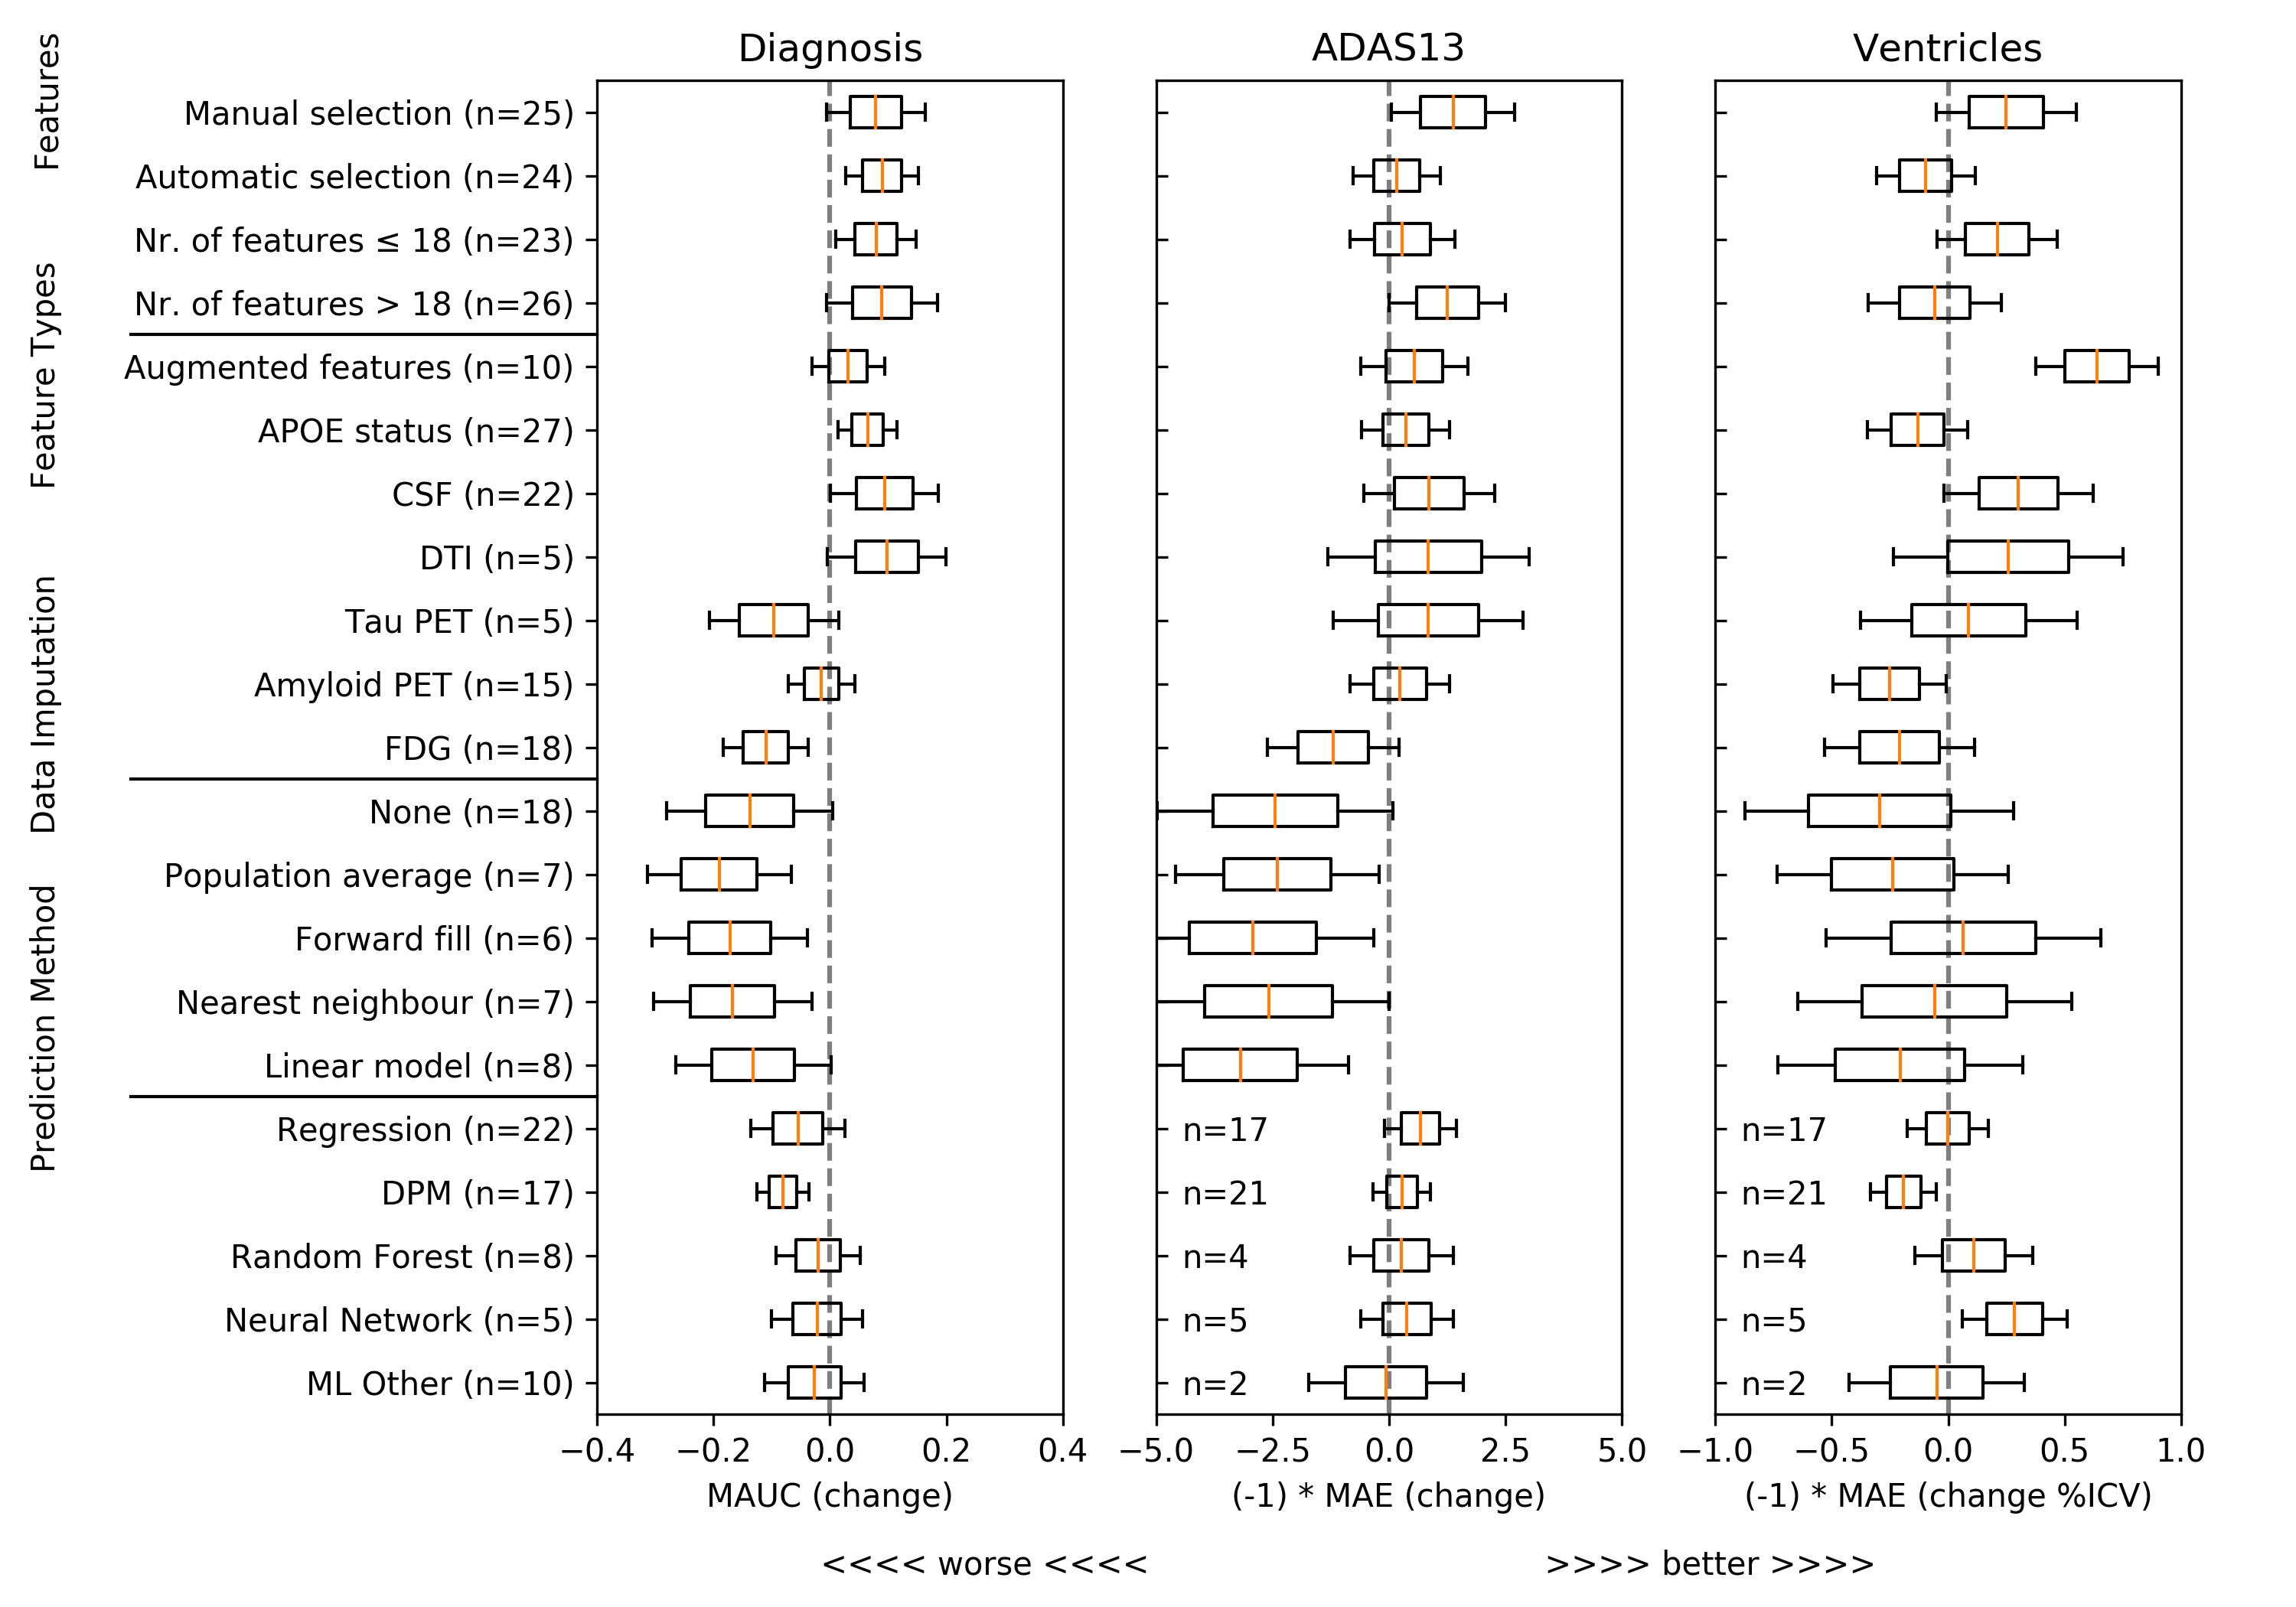
\includegraphics[width=\textwidth]{methodsMetaAnalysisAll}};
\node at (-1.0,1.2)[draw, red,line width=1pt,circle,minimum size=1cm]{};
\node at (3.75,1.8)[draw, red,line width=1pt,circle,minimum size=1cm]{};
\end{tikzpicture}
\end{figure}

\end{column}

\end{columns}

\end{frame}


% \begin{frame}
% \frametitle{Takeaway 7: In simulated clinical trial, a-priori stratification using TADPOLE predictions considerably increases significance}
% 
% 
% \begin{figure}
% \centering
%  \includegraphics[width=\textwidth]{../../generated/resAll-0}
% \end{figure}
% 
% \end{frame}



% \begin{frame}{Conclusions}
%  
% \begin{columns}[t]
% \begin{column}[t]{0.5\textwidth}
% \begin{itemize}
%   \onslide<1-> \item Which biomarkers can we predict, and which we cannot? 
%   
%   \begin{itemize}
%   \item YES: diagnosis, ventricles
%   \item NO: cognition (ADAS-Cog 13)
% \end{itemize}    
%   
%   \vspace{2em}
%    
%  
%   \onslide<2-> \item What is the state-of-the-art in Alzheimer's prediction?
%   
%   \begin{tabular}{|c | c | c|}
%   \hline
%   Diagnosis MAUC & Cognition MAE & Ventricles MAE\\
%   \hline
%   0.931 & - & 0.41\\
%   \hline
%   \end{tabular}
%   
%   
%   \vspace{2em}
%   
%   \onslide<3-> \item What are the winner algorithms? Should I use deep learning or not?
%   
%   \begin{itemize}
%   \item No clear winner
%    \item Clinical diagnosis: gradient boosting
%    \item Ventricle MAE: disease progression model
%    \item Best deep learning algo: 5th place
%   \end{itemize}
%   
%   \vspace{2em}
% \end{itemize}  
%   
% \end{column}
% \begin{column}[t]{0.5\textwidth}
% % \vspace{0.2em}
% \begin{itemize}
% %   \onslide<4-> \item Consensus (averaging over teams' predictions): good or not?
% %   \begin{itemize}
% %   \item Consensus achieves top results
% %   \item Diagnosis: 11\% better  than TADPOLE best for cognition
% %   \item Ventricles: 8\% better than TADPOLE best 
% % \end{itemize}    
% %   
% %   \vspace{2em}
%   
%   \onslide<5-> \item Features: which ones are most informative? Do I need to pre-process those DTI scans, are MRIs not enough?
%    
%  \begin{itemize}
%  \item Diagnosis: CSF and DTI
%  \item Ventricles: Augmented features
% \end{itemize}  
%   
%   \vspace{2em}
%  
%   
%   \onslide<6-> \item How well do algorithms work on "real data", mimicking clinical trials
%  \begin{itemize}
%   \item minor loss in prediction performance
%   \item  0.917 vs 0.931 on diagnosis prediction
% \end{itemize}   
%   
%  \end{itemize}
% 
% \end{column}
% \end{columns} 
%  
%  
%  
% \end{frame}


\begin{frame}
\frametitle{Next steps}

\begin{figure}
 
\begin{subfigure}{0.6\textwidth}
 
\begin{itemize}
% \item Manuscript in preparation

% \vspace{3em}

\item TADPOLE SHARE: \url{https://tadpole-share.github.io/}
    \begin{itemize}
    \item share methods for validation and further development
    \item 11 teams already sharing
    \item Lead by Esther Bron: e.bron@erasmusmc.nl
    \end{itemize}

\vspace{3em}

\item AAIC 2020 special symposium
% \begin{itemize}
%   \item teams will present results
% \end{itemize}

\vspace{3em}

\item Follow-on evaluations as more ADNI data becomes available

\vspace{3em}

\item Challenge still ongoing, D4 leaderboard now live

\end{itemize}

\end{subfigure}
\begin{subfigure}{0.3\textwidth}
 \centering
 \vspace{-4em}
 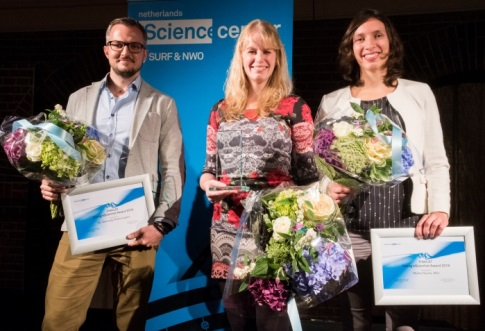
\includegraphics[width=\textwidth]{esther_tadpoleshare}
 
\includegraphics[width=\textwidth]{netherlands_escience}
\end{subfigure}
\end{figure}

\end{frame}


\begin{frame}
\frametitle{Overview}

%% new slide

\begin{figure}
\centering

{\transparent{0.4}
\ovEBM
\ovVWDPM

\ovDKT
\ovTadpole}

\ovPainter



\end{figure}
\end{frame}



% 
% \begin{frame}[label=current]
% \frametitle{Acknowledgements}
% 
% % 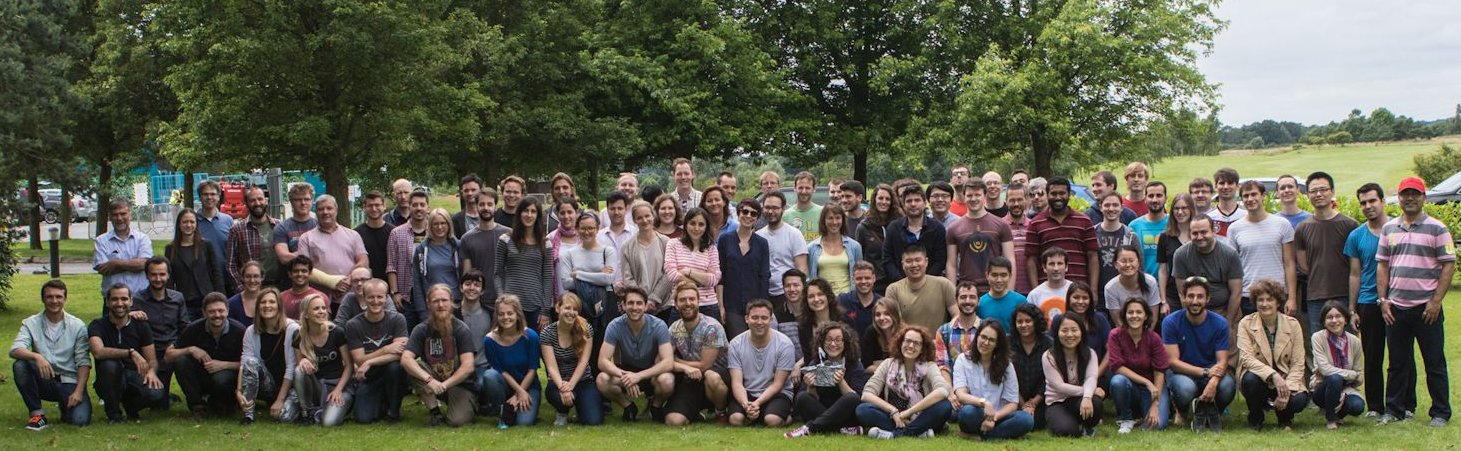
\includegraphics[width=\textwidth,trim=0 0 0 150, clip]{cmic_away_day}
% \newcommand{\heiLogoFund}{1.5cm}
%      
% \begin{columns}[T]
%    \begin{column}{.5\textwidth}
%         
%        \begin{itemize}
%        \item  \textbf{Challenge Participants}\\
%         \vspace{2em}
%         
%        \item  \textbf{Sponsors}\\
%        
%         \vspace{2em}
%         
%         
\includegraphics[height=\heiLogoFund]{alzsoc_logo}
%         
\includegraphics[height=\heiLogoFund]{alzresuk_logo}
%         
%         
\includegraphics[height=0.9cm]{alzassoc_logo}
%         
% %        \item \textbf{Organisers and advisors}
% %        \begin{itemize}
% %        \item Daniel Alexander
% %        \item Neil Oxtoby
% %        \item Polina Golland
% %        \item Esther Bron
% %        \item Stefan Klein
% %        \item Alexandra Young
% %        \item Sara Garbarino
% %        \item Frederik Barkhof
% %        \item Nick Fox
% %        \item EuroPOND consortium
% %        \item LONI team at USC
% %        \item ADNI Consortium
% %        \end{itemize}
%     
%      \end{itemize}
% 
%     
% %     \includegraphics[scale=1]{pondLogo.png}  
%   \end{column}
%     
%     
%     \begin{column}{.5\textwidth}
% %     \begin{center}
% %     \textbf{Project Supervisors}
% %     \end{center}
% %     \vspace{-2em}
%       \begin{figure}
% %       \begin{subfigure}{0.3\textwidth}
% %       \centering
% %       Daniel Alexander
% %       \includegraphics[height=2cm]{Danny-Alexander.jpeg}  
% %       \end{subfigure}
% % 	\begin{subfigure}{0.3\textwidth}
% % 	\centering
% %       Sebastian Crutch
% %       \includegraphics[height=2cm]{Seb_Crutch_photo.JPG}  
% %       \end{subfigure}
% %   \begin{subfigure}{0.3\textwidth}
% % 	\centering
% %       Polina Golland
% %       \includegraphics[height=2cm, trim=0 00 0 0,clip]{polina}  
% %       \end{subfigure}
%       
%     \begin{itemize}
%     \item \textbf{Funders}
%     \end{itemize}
% 
%     %\vspace{-2em}
% 
%     
%     \vspace{2em}
%     \includegraphics[height=\heiLogoFund]{eufp7_logo}
%     
%     \includegraphics[height=\heiLogoFund]{epsrc_logo}\hspace{2em}
%     \includegraphics[height=\heiLogoFund]{nac_logo}
%     
%     
%     
%        
%       \vspace{2em}
% 
% \end{figure}
%     
% \end{column}
% \end{columns}
%  
% 
% \end{frame}


% \end{comment}

\end{document}



